\PassOptionsToPackage{unicode=true}{hyperref} % options for packages loaded elsewhere
\PassOptionsToPackage{hyphens}{url}
\PassOptionsToPackage{dvipsnames,svgnames*,x11names*}{xcolor}
%
\documentclass[12pt,]{book}
\usepackage{lmodern}
\usepackage{amssymb,amsmath}
\usepackage{ifxetex,ifluatex}
\usepackage{fixltx2e} % provides \textsubscript
\ifnum 0\ifxetex 1\fi\ifluatex 1\fi=0 % if pdftex
  \usepackage[T1]{fontenc}
  \usepackage[utf8]{inputenc}
  \usepackage{textcomp} % provides euro and other symbols
\else % if luatex or xelatex
  \usepackage{unicode-math}
  \defaultfontfeatures{Ligatures=TeX,Scale=MatchLowercase}
\fi
% use upquote if available, for straight quotes in verbatim environments
\IfFileExists{upquote.sty}{\usepackage{upquote}}{}
% use microtype if available
\IfFileExists{microtype.sty}{%
\usepackage[]{microtype}
\UseMicrotypeSet[protrusion]{basicmath} % disable protrusion for tt fonts
}{}
\IfFileExists{parskip.sty}{%
\usepackage{parskip}
}{% else
\setlength{\parindent}{0pt}
\setlength{\parskip}{6pt plus 2pt minus 1pt}
}
\usepackage{xcolor}
\usepackage{hyperref}
\hypersetup{
            colorlinks=true,
            linkcolor=Maroon,
            filecolor=Maroon,
            citecolor=Blue,
            urlcolor=Blue,
            breaklinks=true}
\urlstyle{same}  % don't use monospace font for urls
\usepackage[margin=1in]{geometry}
\usepackage{color}
\usepackage{fancyvrb}
\newcommand{\VerbBar}{|}
\newcommand{\VERB}{\Verb[commandchars=\\\{\}]}
\DefineVerbatimEnvironment{Highlighting}{Verbatim}{commandchars=\\\{\}}
% Add ',fontsize=\small' for more characters per line
\usepackage{framed}
\definecolor{shadecolor}{RGB}{248,248,248}
\newenvironment{Shaded}{\begin{snugshade}}{\end{snugshade}}
\newcommand{\AlertTok}[1]{\textcolor[rgb]{0.94,0.16,0.16}{#1}}
\newcommand{\AnnotationTok}[1]{\textcolor[rgb]{0.56,0.35,0.01}{\textbf{\textit{#1}}}}
\newcommand{\AttributeTok}[1]{\textcolor[rgb]{0.77,0.63,0.00}{#1}}
\newcommand{\BaseNTok}[1]{\textcolor[rgb]{0.00,0.00,0.81}{#1}}
\newcommand{\BuiltInTok}[1]{#1}
\newcommand{\CharTok}[1]{\textcolor[rgb]{0.31,0.60,0.02}{#1}}
\newcommand{\CommentTok}[1]{\textcolor[rgb]{0.56,0.35,0.01}{\textit{#1}}}
\newcommand{\CommentVarTok}[1]{\textcolor[rgb]{0.56,0.35,0.01}{\textbf{\textit{#1}}}}
\newcommand{\ConstantTok}[1]{\textcolor[rgb]{0.00,0.00,0.00}{#1}}
\newcommand{\ControlFlowTok}[1]{\textcolor[rgb]{0.13,0.29,0.53}{\textbf{#1}}}
\newcommand{\DataTypeTok}[1]{\textcolor[rgb]{0.13,0.29,0.53}{#1}}
\newcommand{\DecValTok}[1]{\textcolor[rgb]{0.00,0.00,0.81}{#1}}
\newcommand{\DocumentationTok}[1]{\textcolor[rgb]{0.56,0.35,0.01}{\textbf{\textit{#1}}}}
\newcommand{\ErrorTok}[1]{\textcolor[rgb]{0.64,0.00,0.00}{\textbf{#1}}}
\newcommand{\ExtensionTok}[1]{#1}
\newcommand{\FloatTok}[1]{\textcolor[rgb]{0.00,0.00,0.81}{#1}}
\newcommand{\FunctionTok}[1]{\textcolor[rgb]{0.00,0.00,0.00}{#1}}
\newcommand{\ImportTok}[1]{#1}
\newcommand{\InformationTok}[1]{\textcolor[rgb]{0.56,0.35,0.01}{\textbf{\textit{#1}}}}
\newcommand{\KeywordTok}[1]{\textcolor[rgb]{0.13,0.29,0.53}{\textbf{#1}}}
\newcommand{\NormalTok}[1]{#1}
\newcommand{\OperatorTok}[1]{\textcolor[rgb]{0.81,0.36,0.00}{\textbf{#1}}}
\newcommand{\OtherTok}[1]{\textcolor[rgb]{0.56,0.35,0.01}{#1}}
\newcommand{\PreprocessorTok}[1]{\textcolor[rgb]{0.56,0.35,0.01}{\textit{#1}}}
\newcommand{\RegionMarkerTok}[1]{#1}
\newcommand{\SpecialCharTok}[1]{\textcolor[rgb]{0.00,0.00,0.00}{#1}}
\newcommand{\SpecialStringTok}[1]{\textcolor[rgb]{0.31,0.60,0.02}{#1}}
\newcommand{\StringTok}[1]{\textcolor[rgb]{0.31,0.60,0.02}{#1}}
\newcommand{\VariableTok}[1]{\textcolor[rgb]{0.00,0.00,0.00}{#1}}
\newcommand{\VerbatimStringTok}[1]{\textcolor[rgb]{0.31,0.60,0.02}{#1}}
\newcommand{\WarningTok}[1]{\textcolor[rgb]{0.56,0.35,0.01}{\textbf{\textit{#1}}}}
\usepackage{longtable,booktabs}
% Fix footnotes in tables (requires footnote package)
\IfFileExists{footnote.sty}{\usepackage{footnote}\makesavenoteenv{longtable}}{}
\usepackage{graphicx,grffile}
\makeatletter
\def\maxwidth{\ifdim\Gin@nat@width>\linewidth\linewidth\else\Gin@nat@width\fi}
\def\maxheight{\ifdim\Gin@nat@height>\textheight\textheight\else\Gin@nat@height\fi}
\makeatother
% Scale images if necessary, so that they will not overflow the page
% margins by default, and it is still possible to overwrite the defaults
% using explicit options in \includegraphics[width, height, ...]{}
\setkeys{Gin}{width=\maxwidth,height=\maxheight,keepaspectratio}
\setlength{\emergencystretch}{3em}  % prevent overfull lines
\providecommand{\tightlist}{%
  \setlength{\itemsep}{0pt}\setlength{\parskip}{0pt}}
\setcounter{secnumdepth}{5}
% Redefines (sub)paragraphs to behave more like sections
\ifx\paragraph\undefined\else
\let\oldparagraph\paragraph
\renewcommand{\paragraph}[1]{\oldparagraph{#1}\mbox{}}
\fi
\ifx\subparagraph\undefined\else
\let\oldsubparagraph\subparagraph
\renewcommand{\subparagraph}[1]{\oldsubparagraph{#1}\mbox{}}
\fi

% set default figure placement to htbp
\makeatletter
\def\fps@figure{htbp}
\makeatother

\usepackage{booktabs}
\usepackage{amsthm}
\makeatletter
\def\thm@space@setup{%
  \thm@preskip=8pt plus 2pt minus 4pt
  \thm@postskip=\thm@preskip
}
\makeatother
%\usepackage[T1]{fontenc}
%\usepackage{textcomp}
%\usepackage{fontspec}
%\mainfont[Ligatures=TeX]{Lato}
\usepackage{fancyhdr}
\pagestyle{fancy}
\fancyhf{}
\fancyfoot[LE,LO]{
\includegraphics[width=2cm]{Images/egap-logo.png}}
\fancyfoot[RE,RO]{\thepage}
%\usepackage{libertinus}
%\usepackage[autocite=plain,style=verbose,citetracker=false]{biblatex}
\usepackage[autocite=plain,citestyle=verbose]{biblatex}
\usepackage{caption}
\usepackage[]{biblatex}
\addbibresource{learningdays-book.bib}

\title{The Theory and Practice of Field Experiments:\\
An Introduction from the EGAP Learning Days}
\author{Jake Bowers,\footnote{Author order randomized. \url{https://jakebowers.org}} Maarten Voors,\footnote{\url{https://sites.google.com/site/maartenvoors/}} and Nahomi Ichino\footnote{\url{https://nahomi.github.io/}}~\\
(\href{https://egap.github.io/theory_and_practice_of_field_experiments_spanish/}{Spanish translation by Lily Medina})\\
(\href{https://egap.github.io/theory_and_practice_of_field_experiments_french/}{French translation by Alyssa Heinze})}
\date{January 12, 2023}

\begin{document}
\maketitle

\captionsetup[table]{list=no}
\captionsetup[figure]{list=no}

{
\hypersetup{linkcolor=}
\setcounter{tocdepth}{1}
\tableofcontents
}
\hypertarget{introduction}{%
\chapter{Introduction}\label{introduction}}

Over the past decade, \href{http://egap.org/}{Evidence in Governance and Politics (EGAP)} has organized \href{https://egap.org/learning-days/}{Learning Days} workshops with the aim of building experimental social-science research capacity among principal investigators (PIs) -- both researchers and practitioners -- in Africa and Latin America. By sharing the practical and statistical methods of randomized field experiments with workshop participants, the Learning Days effort hopes to identify and nurture researcher networks around the world and to create strong, productive connections between these researchers and EGAP members.

The Learning Days workshops are a combination of design clinics, research presentations, guided work with statistical software, and topical lectures by a small group of instructors, largely professors and PhD students from the EGAP network. The workshops focus on methods for the design and analysis of randomized experiments in the field rather than on randomized experiments in the lab or non-randomized studies.

\textbf{This book} grew out of a desire to share the materials we developed for the Learning Days. The current version is written primarily for \textbf{instructors and organizers} of similar workshops and courses aimed at PIs --- i.e., professors, post-doctoral fellows, PhD students, and NGO/government agency evaluators --- who will implement randomized studies of programs related to institutions, governance, and development. Much of the material will also be useful as a refresher for past participants of the Learning Days workshops.

This book is a comprehensive overview of causal inference methods for researchers developing an experimental research design. It is organized in \textbf{modules} and covers topics such as causal inference, randomization, hypothesis testing, estimands, estimators, statistical power, measurement, threats to internal validity, and the ethics of experimentation. The modules appear in the order the Learning Days instructors have found most useful. However, the modules are linked to one another and can be reordered to suit your needs as an instructor. In the appendix, we include some course preliminaries including a \href{glossary-of-terms.html}{glossary of terms} and an \href{introduction-to-r-and-rstudio.html}{introduction to R and RStudio}.

The book includes \textbf{slides} on the core content, the \href{researchdesignform.html}{EGAP Research Design Form}, and \textbf{references} to research examples and slides used in previous Learning Days. This material builds significantly on and links to EGAP's work on methodology, summarized in the \href{https://egap.org/methods-guides/}{EGAP Methods Guides}. We have made significant extensions to the past Learning Days' materials on hypothesis testing, estimation, and statistical power and added new modules on the research design process, measurement, and ethical considerations. The slides and modules presented here contain too much information to be covered in a single week, the usual length of a Learning Days workshop. We have chosen to present more rather than less information, however, to help instructors tailor their courses to their specific audiences.

\hypertarget{how-to-use-the-book}{%
\section{How to use the book}\label{how-to-use-the-book}}

To gain the most benefit from this book, please have \href{https://cran.r-project.org/}{R} and \href{https://www.rstudio.com/products/rstudio/download/}{RStudio} installed on your machine. In fact, the slides assume that you will use Rmarkdown to adapt them for your own purposes.

To get going with R, see the module \href{introduction-to-r-and-rstudio.html}{Introduction to R and RStudio}.

You can copy this book or parts thereof (e.g., slides, etc.) either by using the Download button on the front page of \url{http://github.com/egap/theory_and_practice_of_field_experiments} or by using github directly (by forking this repository).

We are happy for anyone to use the materials as long as EGAP is attributed. See Creative Commons Attribution-ShareAlike 4.0 International License for the precise terms.

\hypertarget{we-would-love-to-hear-from-you}{%
\section{We would love to hear from you!}\label{we-would-love-to-hear-from-you}}

If you have any questions, feedback or have organized your own event, please get in touch! Simply post an issue on \href{https://github.com/egap/theory_and_practice_of_field_experiments/issues}{Github} or make comments using hypothes.is in your browser and let us know via email, \href{mailto:admin@egap.org}{\nolinkurl{admin@egap.org}}. We'll periodically go through the comments.

\hypertarget{acknowledgments}{%
\section{Acknowledgments}\label{acknowledgments}}

The materials included in this book have been developed over the past years by various Learning Days instructors. These include (in alphabetical order) Jake Bowers, Jasper Cooper, Ana De la O, Lindsay Dolan, Natalia Garbiras Díaz, Macartan Humphreys, Nahomi Ichino, Salif Jaiteh, Gareth Nellis, Dan Nielson, Rafael Piñeiro, Fernando Rosenblatt, Tara Slough, Peter van der Windt and Maarten Voors. We thank Natalia Garbiras Díaz, Macartan Humphreys, Anghella Brigeth Rosero Rodriguez, and Tara Slough in particular for comments on an early draft of the book. We also thank
Brice Bado, Simon Chauchard, Jasper Cooper, Simone Dietrich, Thad Dunning, Jessica Gottlieb, Macartan Humphreys, Julien Labonne, Ambaliou Olounlade, Daniel Rubenson, and Saloua Zerhouni for their help in reviewing the French translation and Rosario Aguilar, Ana De la O, Pablo Egaña del Sol, Omar Garcia Ponce, Paul Lagunes, Luis Maldonado, Fernando Martel Garcia, Paula Muñoz, Raul Pacheco-Vega, Rafael Piñiero, Pablo Querubin, Mauricio Romero, Fernando Rosenblatt, Santiago Saavedra, Lucía Tiscornia, Santiago Tobón, and Juan Vargas for their help in reviewing the Spanish translation of these materials.

At EGAP, Matt Lisiecki, Ingrid Lee, Goldie Negelev, Max Mendez-Back and others have provided wonderful support. Learning Days have been generously funded by the Hewlett Foundation and supported by institutions around the world including the African School of Economics (Benin), Universidad Diego Portales (Chile), Universidad de los Andes (Colombia), Ghana Center for Democratic Development (Ghana), Mercy Corps (Guatemala), Invest in Knowledge (Malawi), NYU Abu Dhabi (UAE), Universidad Católica del Uruguay (Uruguay).

\hypertarget{the-research-design-process}{%
\chapter{The Research Design Process}\label{the-research-design-process}}

This book aims to help you understand and design randomized field experiments. But before we dive into the details of research design, we need a good research question -- a question that will advance knowledge or help make a policy decision or both. There is no simple recipe for finding or developing a good scientific or policy question, but our theories are important for articulating good questions that underlie impactful research. After formulating our question, we develop the best design possible within our resource constraints, using our knowledge of causal inference and statistics from the modules that follow.

This module introduces the \href{https://egap.github.io/learningdays-resources/Exercises/design-form.Rmd}{EGAP Research Design
Form}, a checklist to guide you through the many stages of the research process. The Learning Days workshops are organized around the Research Design Form. We also point you towards the \href{http://declaredesign.org}{DeclareDesign} software package to explore the implications of different choices we could make for our research designs. Finally, this module discusses pre-analysis plans and pre-registration. When plan our analyses and make these plans public, we improve our chances of persuading others with our results.

\hypertarget{core-content}{%
\section{Core Content}\label{core-content}}

\begin{itemize}
\item
  A \textbf{good research question} advances science and/or is a question the answer to which will inform a policy decision.
\item
  Certain \textbf{research designs} are better able to address certain questions. We want to choose the design that best answers our key questions within our constraints.
\item
  The questions we ask arise --- often implicitly --- from our values and from our understanding about how the world works. These \textbf{theories} make our questions relevant. And the experiments that we execute teach us about the theory. That is, we hope that the evidence and data arising from these research designs improve our understanding.
\item
  Core components of a research design
\item
  Introduce core components of the \href{https://egap.github.io/learningdays-resources/Exercises/design-form.html}{EGAP Research Design Form}.
\item
  Introduce a research design software package, \href{http://declaredesign.org}{DeclareDesign}.
\item
  The move in social science towards the \textbf{review of designs, rather than outcomes}.
\item
  \textbf{Pre-registration} -- what it is, and why and how we should do it.
\end{itemize}

\hypertarget{slides}{%
\section{Slides}\label{slides}}

Below are slides with the core content that we cover in our lecture on research design. You can directly use these slides or make your own local copy and edit.

\begin{itemize}
\item
  \href{https://egap.github.io/learningdays-resources/Slides/researchdesignform-slides.Rmd}{R Markdown Source}
\item
  \href{https://egap.github.io/learningdays-resources/Slides/researchdesignform-slides.pdf}{PDF Version}
\item
  \href{https://egap.github.io/learningdays-resources/Slides/researchdesignform-slides.html}{HTML Version}
\end{itemize}

You can also see the slides used in previous EGAP Learning Days:

\begin{itemize}
\item
  \href{https://egap.github.io/learningdays-resources/Slides/Examples/declare_design-montevideo.pdf}{The DeclareDesign presentation from EGAP Learning Days at Universidad Católica del Uruguay, Montevideo, March 2018}
\item
  \href{https://egap.github.io/learningdays-resources/Slides/Examples/declare_design-malawi.pdf}{The DeclareDesign presentation from EGAP Learning Days in Salima, Malawi, February 2017}
\item
  \href{https://egap.github.io/learningdays-resources/Slides/Examples/declare_design-santiago.pdf}{The DeclareDesign presentation from EGAP Learning Days at Universidad Diego Portales in Santiago, Chile, May 2016}
\end{itemize}

You can also see slides for Design Talks in previous EGAP Learning Days, where presenters focus on issues that come up in designing the research, rather than the results:

\begin{itemize}
\item
  \href{https://egap.github.io/learningdays-resources/Slides/Examples/research_design_2-benin.pdf}{Design Talk from EGAP Learning Days at the African School of Economics, Benin, March 2018}
\item
  \href{https://egap.github.io/learningdays-resources/Slides/Examples/research_design_1-montevideo.pdf}{Design Talk 1 from EGAP Learning Days at Universidad Católica del Uruguay, Montevideo, March 2018}
\item
  \href{https://egap.github.io/learningdays-resources/Slides/Examples/research_design_2-montevideo.pdf}{Design Talk 2 from EGAP Learning Days at Universidad Católica del Uruguay, Montevideo, March 2018}
\item
  \href{https://egap.github.io/learningdays-resources/Slides/Examples/research_design_3-montevideo.pdf}{Design Talk 3 from EGAP Learning Days at Universidad Católica del Uruguay, Montevideo, March 2018}
\item
  \href{https://egap.github.io/learningdays-resources/Slides/Examples/research_design_1-santiago.pdf}{Design Talk 1 from EGAP Learning Days at Universidad Diego Portales in Santiago, Chile, May 2016}
\item
  \href{https://egap.github.io/learningdays-resources/Slides/Examples/research_design_2-santiago.pdf}{Design Talk 2 from EGAP Learning Days at Universidad Diego Portales in Santiago, Chile, May 2016}
\item
  \href{https://egap.github.io/learningdays-resources/Slides/Examples/research_design_3-santiago.pdf}{Design Talk 3 from EGAP Learning Days at Universidad Diego Portales in Santiago, Chile, May 2016}
\item
  \href{https://egap.github.io/learningdays-resources/Slides/Examples/research_design-guatemala.pdf}{Design Talk from EGAP Learning Days in Guatemala City, Guatemala, August 2017}
\end{itemize}

\hypertarget{design-form-and-pre-registration}{%
\section{Design Form and Pre-registration}\label{design-form-and-pre-registration}}

\begin{itemize}
\item
  \href{https://egap.github.io/learningdays-resources/Exercises/design-form.html}{EGAP Research Design Form}. A checklist we created for the Learning Days to guide you through the stages of the research process.

  \begin{itemize}
  \item
    \href{https://egap.github.io/learningdays-resources/Exercises/design-form.docx}{Docx Version}
  \item
    \href{https://egap.github.io/learningdays-resources/Exercises/design-form.pdf}{PDF Version}
  \item
    \href{https://egap.github.io/learningdays-resources/Exercises/design-form.html}{HTML Version}
  \end{itemize}
\item
  Links to repositories for pre-registration/pre-analysis plans:

  \begin{itemize}
  \item
    EGAP registry, hosted by OSF (\url{https://egap.org/registry/})
  \item
    AEA RCT registry (\url{https://www.socialscienceregistry.org/})
  \item
    OSF (\url{https://osf.io/registries})
  \end{itemize}
\item
  Examples of other pre-registrations/pre-analysis plans:

  \begin{itemize}
  \item
    SMS Messages in Mozambique from the \href{https://oes.gsa.gov/projects/sms-mozambique/}{US Federal Government}
  \item
    Police Body-Cameras from the \href{https://osf.io/472zh}{Lab @ DC}
  \end{itemize}
\end{itemize}

\hypertarget{resources}{%
\section{Resources}\label{resources}}

\hypertarget{egap-methods-guides}{%
\subsection{EGAP Methods Guides}\label{egap-methods-guides}}

\begin{itemize}
\item
  EGAP Methods Guide \href{https://egap.org/resource/10-things-to-know-about-pre-analysis-plans/}{10 Things to Know about Pre-Analysis Plans}
\item
  EGAP Methods Guide \href{https://egap.org/resource/10-things-to-know-about-measurement-in-experiments/}{10 Things to Know about Measurement in Experiments}
\end{itemize}

\hypertarget{books-chapters-and-articles}{%
\subsection{Books, Chapters, and Articles}\label{books-chapters-and-articles}}

\begin{itemize}
\item
  \href{https://oes.gsa.gov/assets/files/preregistration-as-a-tool-in-federal-evaluation.pdf}{Preregistration as a Tool for Strengthening Federal Evaluation}. A white paper from the US Government's Office of Evaluation Sciences. You can also see examples of their pre-analysis plans on all of \href{https://oes.gsa.gov/work/}{their field experiment pages}.
\item
  \autocite{christensen_transparent_2019}. The book summarizes new approaches in social science research on transparency and reproducibility.
\item
  \autocite{gerber_field_2012}. Chapter 12 includes some examples of experimental research designs.
\end{itemize}

\hypertarget{tools}{%
\subsection{Tools}\label{tools}}

\begin{itemize}
\tightlist
\item
  \href{https://declaredesign.org/}{DeclareDesign}, an exciting and comprehensive set of software tools for describing, assessing, and conducting empirical research.
\end{itemize}

\hypertarget{causal-inference}{%
\chapter{Causal Inference}\label{causal-inference}}

Much of social science is about causality. We might ask questions like whether \href{https://egap.org/resource/electoral-administration-in-kenya/}{voter registration increases political participation}, whether \href{https://egap.org/resource/does-bottom-up-accountability-work-evidence-from-uganda/}{bottom-up accountability can improve health outcomes}, or whether \href{https://egap.org/resource/brief-70-how-personal-narratives-reduce-negative-attitudes-towards-immigrants-in-kenya/}{personal narratives of immigrants help reduce prejudicial attitudes towards them}.

Over the past decade, social science has become much more serious about how causal claims are made, building on a long history of work on causality dating back to the classic writings of \protect\hyperlink{causalinference-classics}{Fisher and Rubin}. We make greater use of experiments, and randomization has become the gold standard for addressing causal questions.

In this module, we introduce the counterfactual approach to causal inference and how statements with causal claims can be interpreted. We introduce the potential outcome framework and how random assignment helps us make claims about what would have happened in the absence of the policy, action or program we study. We discuss the three core assumptions for causal inference: random assignment of subjects to treatment, non-interference, and excludability.

\hypertarget{core-content-1}{%
\section{Core Content}\label{core-content-1}}

\begin{itemize}
\item
  What do we mean when we say \textbf{``cause''}? And why does it matter to be clear about the meaning of causal claims?
\item
  An introduction to \textbf{potential outcomes} as a way to think about alternative states of the world.
\item
  \textbf{Randomization} helps us learn about counterfactual causal claims in a particularly useful way.
\item
  The three key \textbf{core assumptions} for causal inference: random assignment of subjects to treatment, non-interference, and excludability.
\item
  Comparison of randomized studies with observational studies.
\item
  Randomization brings high internal validity, but it can't promise \textbf{external validity}.
\item
  Your causal question is closely linked so your \href{the-research-design-process.html}{research design}.
\end{itemize}

\hypertarget{slides-1}{%
\section{Slides}\label{slides-1}}

Below are slides with the core content that we cover in our lecture on causality. You can directly use these slides or make your own local copy and edit.

\begin{itemize}
\item
  \href{https://egap.github.io/learningdays-resources/Slides/causalinference-slides.Rmd}{R Markdown Source}
\item
  \href{https://egap.github.io/learningdays-resources/Slides/causalinference-slides.pdf}{PDF Version}
\item
  \href{https://egap.github.io/learningdays-resources/Slides/causalinference-slides.html}{HTML Version}
\end{itemize}

You can also see the slides used in previous EGAP Learning Days:

\begin{itemize}
\item
  \href{https://egap.github.io/learningdays-resources/Slides/Examples/causality-benin.pdf}{The causal inference presentation from EGAP Learning Days at the African School of Economics, Abomey-Calavi, June 2019}
\item
  \href{https://egap.github.io/learningdays-resources/Slides/Examples/causality-bogota.pdf}{The causal inference presentation from EGAP Learning Days at Universidad de Los Andes, Bogotá, April 2019}
\item
  \href{https://egap.github.io/learningdays-resources/Slides/Examples/causality-montevideo.pdf}{The causal inference presentation from EGAP Learning Days at Universidad Católica del Uruguay, Montevideo, March 2018}
\item
  \href{https://egap.github.io/learningdays-resources/Slides/Examples/causality-guatemala.pdf}{The causal inference presentation from EGAP Learning Days in Guatemala City, Guatemala, August 2017}
\item
  \href{https://egap.github.io/learningdays-resources/Slides/Examples/intro_experiments-guatemala.pdf}{The introduction to experiments presentation from EGAP Learning Days in Guatemala City, Guatemala, August 2017}
\item
  \href{https://egap.github.io/learningdays-resources/Slides/Examples/causality-malawi.pdf}{The causal inference presentation from EGAP Learning Days in Salima, Malawi, February 2017}
\item
  \href{https://egap.github.io/learningdays-resources/Slides/Examples/causality-santiago.pdf}{The causal inference presentation from EGAP Learning Days at Universidad Diego Portales in Santiago, Chile, May 2016}
\end{itemize}

\hypertarget{resources-1}{%
\section{Resources}\label{resources-1}}

\hypertarget{egap-methods-guides-1}{%
\subsection{EGAP Methods Guides}\label{egap-methods-guides-1}}

\begin{itemize}
\item
  EGAP Methods Guide \href{https://egap.org/resource/10-things-to-know-about-causal-inference/}{10 Things You Need to Know about Causal Inference}
\item
  EGAP Methods Guide \href{https://egap.org/resource/10-strategies-for-figuring-out-if-x-caused-y/}{10 Strategies for Figuring Out If X Caused Y}
\item
  EGAP Methods Guide \href{https://egap.org/resource/10-things-mechanisms/}{10 Things You Need to Know about Mechanisms}
\item
  EGAP Methods Guide \href{https://egap.org/resource/10-things-to-know-about-external-validity/}{10 Things to Know About External Validity}
\end{itemize}

\hypertarget{causalinference-cites}{%
\subsection{Books, Chapters, and Articles}\label{causalinference-cites}}

\hypertarget{causalinference-classics}{%
\subsubsection{Classics}\label{causalinference-classics}}

\begin{itemize}
\item
  \autocite{fisher_design_1935}. Fisher introduces the idea of randomization and hypothesis testing as a way to learn about causal inference.
\item
  \autocite{rubin:1974}. Rubin introduces the idea of potential outcomes and links counterfactual conceptualizations of causality to statistical inference.
\end{itemize}

\hypertarget{contemporary-overviews}{%
\subsubsection{Contemporary Overviews}\label{contemporary-overviews}}

\begin{itemize}
\item
  \autocite{brady2008causation}.
\item
  \autocite[Chapter 1]{gerber_field_2012}. This book is a great resource for many topics in experimental design.
\item
  \autocite[Chapter 1]{morgan_counterfactuals_2007}. This book includes nice examples of thinking through making causal claims from observational data.
\item
  \autocite{glennerster_running_2013}. This is a great introduction to running field experiments and discusses many examples.
\end{itemize}

\hypertarget{egap-policy-briefs}{%
\subsection{EGAP Policy Briefs}\label{egap-policy-briefs}}

Some examples of causal questions:

\begin{itemize}
\item
  \href{https://egap.org/resource/brief-38-diminishing-the-effectiveness-of-vote-buying-through-voter-education/}{EGAP Policy Brief 38: Are radio voter education campaigns effective in discouraging voters from voting for parties/candidates that engage in vote-buying?}
\item
  \href{https://egap.org/resource/does-information-technology-improve-public-service-delivery-lessons-from-uganda/}{EGAP Policy Brief 51: Can free and anonymous information communication technology strengthen local accountability and improve the delivery of public services?}
\item
  \href{https://egap.org/resource/does-bottom-up-accountability-work-evidence-from-uganda/}{EGAP Policy Brief 58: Can bottom-up accountability generate improvements in health outcomes?}
\item
  \href{https://egap.org/resource/brief-69-bottom-up-accountability-and-public-service-provision-in-brazil/}{EGAP Policy Brief 69: Does bottom-up, citizen-based monitoring improve public service delivery?}
\end{itemize}

\hypertarget{randomization}{%
\chapter{Randomization}\label{randomization}}

The module on \href{causal-inference.html}{causal inference} discussed the crucial role of randomization for drawing valid inferences from a comparison of treated and untreated groups. In this module, we move from theory to the first of many concrete choices for your research design.

We introduce four common ways to randomize treatment -- simple, complete, block, and clustered -- and when these different types of randomization may be available and appropriate. We also cover several popular designs including factorial designs and encouragement designs. The module provides some guidance on implementation, including best practices for checking for balance and ensuring replicability.

\hypertarget{core-content-2}{%
\section{Core Content}\label{core-content-2}}

\begin{itemize}
\item
  What is \textbf{randomization}? Random assignment is \textbf{not} the same as random sampling.
\item
  Four common ways to randomize treatment:

  \begin{itemize}
  \item
    \textbf{Simple}: randomly assign units to treatment (like a coin flip).
  \item
    \textbf{Complete}: within a list of eligible units, a assign a fixed number to receive a treatment (like drawing from a urn).
  \item
    \textbf{Block (or stratified)}: assign treatment within specific strata or blocks, as if you are running an experiment within each block.
  \item
    \textbf{Cluster}: assign groups (clusters) of observations to the same treatment condition.
  \end{itemize}
\item
  Some popular designs:

  \begin{itemize}
  \item
    Randomized \textbf{access}: randomization to availability of a treatment.
  \item
    Randomized \textbf{delayed access}: randomize the timing of access.
  \item
    \textbf{Factorial}: randomize units to combinations of treatment arms.
  \item
    \textbf{Encouragement}: randomize the invitation to receive treatment.
  \end{itemize}
\item
  How do you check whether your randomization produced balance on observables? Typically we conduct randomization tests also known as balance tests using the \(d^2\) omnibus test from \texttt{xBalance} in the \texttt{RItools} package (because it is randomization inference) or approximate this result with an \(F\)-test.
\item
  There are, of course, \textbf{limits to randomization}. We discuss some here and direct you to the module on \href{threats-to-internal-validity-of-randomized-experiments.html}{threats} for more.
\end{itemize}

\hypertarget{slides-2}{%
\section{Slides}\label{slides-2}}

Below are slides with the core content that we cover in our lecture on randomization. You can directly use these slides or make your own local copy and edit.

\begin{itemize}
\item
  \href{https://egap.github.io/learningdays-resources/Slides/randomization-slides.Rmd}{R Markdown Source}
\item
  \href{https://egap.github.io/learningdays-resources/Slides/randomization-slides.pdf}{PDF version}
\item
  \href{https://egap.github.io/learningdays-resources/Slides/randomization-slides.html}{HTML version}
\end{itemize}

The linked files shows how to \href{https://egap.github.io/learningdays-resources/Exercises/randomization-exercises.Rmd}{do replicable randomization in R}. You can also see more examples of randomization in R at \href{https://egap.org/resource/10-things-to-know-about-randomization/}{10 Things You Need to Know About Randomization}.

You can also see the slides used in previous EGAP Learning Days:

\begin{itemize}
\item
  \href{https://egap.github.io/learningdays-resources/Slides/Examples/threats-benin.pdf}{The design issues presentation from EGAP Learning Days at the African School of Economics, Abomey-Calavi, June 2019 (first section reviews randomization designs)}
\item
  \href{https://egap.github.io/learningdays-resources/Slides/Examples/randomization-bogota.pdf}{The randomization presentation from EGAP Learning Days at Universidad de Los Andes, Bogotá, April 2019}
\item
  \href{https://egap.github.io/learningdays-resources/Slides/Examples/randomization-montevideo.pdf}{The randomization presentation from EGAP Learning Days at Universidad Católica del Uruguay, Montevideo, March 2018}
\item
  \href{https://egap.github.io/learningdays-resources/Slides/Examples/randomization-guatemala.pdf}{The randomization presentation from EGAP Learning Days in Guatemala City, Guatemala, August 2017}
\item
  \href{https://egap.github.io/learningdays-resources/Slides/Examples/randomization-malawi.pdf}{The randomization presentation from EGAP Learning Days in Salima, Malawi, February 2017}
\item
  \href{https://egap.github.io/learningdays-resources/Slides/Examples/randomization-santiago.pdf}{The randomization presentation from EGAP Learning Days at Universidad Diego Portales in Santiago, Chile, May 2016}
\end{itemize}

\hypertarget{resources-2}{%
\section{Resources}\label{resources-2}}

\hypertarget{egap-methods-guides-2}{%
\subsection{EGAP Methods Guides}\label{egap-methods-guides-2}}

\begin{itemize}
\item
  EGAP Methods Guide \href{https://egap.org/resource/10-things-to-know-about-randomization/}{10 Things You Need to Know About Randomization}
\item
  EGAP Methods Guide \href{https://egap.org/resource/10-things-to-know-about-cluster-randomization/}{10 Things You Need to Know About Cluster Randomization}
\end{itemize}

\hypertarget{books-chapters-and-articles-1}{%
\subsection{Books, Chapters, and Articles}\label{books-chapters-and-articles-1}}

\begin{itemize}
\item
  \href{https://github.com/acoppock/Green-Lab-SOP}{Standard operating procedures for Don Green's lab at Columbia University}. A comprehensive set of procedures and rules of thumb for conducting experimental studies.
\item
  \autocite{glennerster_running_2013}. Chapter 2 on randomization.
\item
  \autocite{gerber_field_2012}. Chapter 2: Causal Inference and Experimentation
\end{itemize}

\hypertarget{egap-policy-briefs-1}{%
\subsection{EGAP Policy Briefs}\label{egap-policy-briefs-1}}

\emph{Factorial designs}

\begin{itemize}
\item
  \href{https://egap.org/resource/how-media-influence-social-norms-evidence-from-mexico/}{EGAP Policy Brief 57: How Media Influence Social Norms: Evidence from Mexico}
\item
  \href{https://egap.org/resource/does-bottom-up-accountability-work-evidence-from-uganda/}{EGAP Policy Brief 58: Does Bottom-Up Accountability Work?}
\end{itemize}

\emph{Randomizing access}

\begin{itemize}
\tightlist
\item
  \href{https://egap.org/resource/brief-24-reducing-elite-capture-in-the-solomon-islands/}{EGAP Policy Brief 24: Reducing Elite Capture in the Solomon Islands}
\end{itemize}

\emph{Randomizing delayed access}

\begin{itemize}
\item
  \href{https://egap.org/resource/brief-35-reducing-reconvictions-among-released-prisoners/}{EGAP Policy Brief 35: Reducing Reconvictions Among Released Prisoners}
\item
  \href{https://egap.org/resource/reducing-youth-support-for-violence-through-training-and-cash-transfers-in-afghanistan/}{EGAP Policy Brief 60: Reducing Youth Support for Violence through Training and Cash Transfers in Afghanistan}
\end{itemize}

\emph{Cluster randomization}

\begin{itemize}
\tightlist
\item
  \href{https://egap.org/resource/brief-22-getting-out-the-vote/}{EGAP Policy Brief 22: Getting Out the Vote}
\end{itemize}

\emph{Blocked cluster randomization}

\begin{itemize}
\item
  \href{https://egap.org/resource/evidence-from-mexico-the-effect-of-incumbent-malfeasance-revelations/}{EGAP Policy Brief 54: Incumbent Malfeasance Revelations}
\item
  \href{https://egap.org/resource/reporting-corruption-in-nigeria-testing-the-effects-of-norms-nudges/}{EGAP Policy Brief 56: Reporting Corruption}
\end{itemize}

\hypertarget{tools-1}{%
\subsection{Tools}\label{tools-1}}

\begin{itemize}
\tightlist
\item
  \href{https://cran.r-project.org/web/packages/RItools/index.html}{RItools}, a set of tools for randomization-based inference including balance testing.
\end{itemize}

\hypertarget{short-explainer-videos}{%
\subsection{Short Explainer Videos}\label{short-explainer-videos}}

\begin{itemize}
\item
  \href{https://www.youtu.be/02A61b3hxvA}{Randomization vs.~Random Sampling}
\item
  \href{https://www.youtu.be/bL2U9z8hX1k}{Cluster vs.~Block Randomization}
\end{itemize}

\hypertarget{hypothesis-testing}{%
\chapter{Hypothesis Testing}\label{hypothesis-testing}}

We cannot directly observe causal effects because of the \emph{fundamental problem of counterfactual causal inference} (\href{causal-inference.html}{causal inference module}). So how can we learn about these \emph{unobserved causal effects} using what we do observe? In a randomized experiment, we can assess \emph{guesses} or \emph{hypotheses} about the unobserved causal effects by comparing what we observe in a given experiment to what we would observe if we were able to repeat the experimental manipulation and the guess or hypothesis were true.

In this module we introduce hypothesis testing, how it relates to causal inference, \(p\)-values, and what to do when we have multiple hypotheses to test.

\hypertarget{core-content-3}{%
\section{Core Content}\label{core-content-3}}

\begin{itemize}
\item
  What is a \textbf{good hypothesis}?
\item
  The relationship between hypothesis testing and causal inference.
\item
  \textbf{Hypothesis tests}.

  \begin{itemize}
  \item
    Null hypotheses.
  \item
    Estimators versus test statistics.
  \item
    In an experiment, a reference distribution for a hypothesis test comes from the experimental design and the randomization.
  \item
    \(p\)-values and how to interpret the results of hypothesis tests.
  \end{itemize}
\item
  A good hypothesis test should (1) cast doubt on the truth rarely (i.e., have a controlled and low false positive rate), and (2) easily distinguish signal from noise (i.e., cast doubt on falsehoods often; have high statistical power).
\item
  How would we know when our hypothesis test is doing a good job? (\href{statistical-power-and-design-diagnosands.html}{Power analysis} is its own module).

  \begin{itemize}
  \item
    False positive rates.
  \item
    Correct coverage of a confidence interval.
  \item
    Assessing the false positive rate of a hypothesis test for a given design and choice of test statistic; the case of cluster-randomized trials and robust cluster standard errors.
  \end{itemize}
\item
  Be careful when testing \textbf{many hypotheses}, such as when you have more than two treatment arms or you are assessing the effects of a treatment on multiple outcomes. We should be careful to \textbf{adjust the \(p\)-values or confidence intervals} to reflect the number of tests/intervals produced.
\end{itemize}

\hypertarget{slides-3}{%
\section{Slides}\label{slides-3}}

Below are slides with the core content that we cover in our lecture on hypothesis testing. You can directly use these slides or make your own local copy and edit.

\begin{itemize}
\item
  \href{https://egap.github.io/learningdays-resources/Slides/hypothesistesting-slides.Rmd}{R Markdown Source}
\item
  \href{https://egap.github.io/learningdays-resources/Slides/hypothesistesting-slides.pdf}{PDF Version}
\item
  \href{https://egap.github.io/learningdays-resources/Slides/hypothesistesting-slides.html}{HTML Version}
\end{itemize}

You can also see the slides used in previous EGAP Learning Days:

\begin{itemize}
\item
  \href{https://egap.github.io/learningdays-resources/Slides/Examples/hypothesistesting-benin.pdf}{The hypothesis testing presentation from EGAP Learning Days at the African School of Economics, Abomey-Calavi, June 2019}
\item
  \href{https://egap.github.io/learningdays-resources/Slides/Examples/hypothesistesting-bogota.pdf}{The hypothesis testing presentation from EGAP Learning Days at Universidad de Los Andes, Bogotá, April 2019}
\item
  \href{https://egap.github.io/learningdays-resources/Slides/Examples/hypothesistesting-montevideo.pdf}{The hypothesis testing presentation from EGAP Learning Days at Universidad Católica del Uruguay, Montevideo, March 2018}
\item
  \href{https://egap.github.io/learningdays-resources/Slides/Examples/hypothesistesting-guatemala.pdf}{The hypothesis testing presentation from EGAP Learning Days in Guatemala City, Guatemala, August 2017}
\item
  \href{https://egap.github.io/learningdays-resources/Slides/Examples/hypothesistesting-malawi.pdf}{The hypothesis testing presentation from EGAP Learning Days in Salima, Malawi, February 2017}
\item
  \href{https://egap.github.io/learningdays-resources/Slides/Examples/hypothesistesting-santiago.pdf}{The hypothesis testing presentation from EGAP Learning Days at Universidad Diego Portales in Santiago, Chile, May 2016}
\end{itemize}

\hypertarget{resources-3}{%
\section{Resources}\label{resources-3}}

\hypertarget{egap-methods-guides-3}{%
\subsection{EGAP Methods Guides}\label{egap-methods-guides-3}}

\begin{itemize}
\item
  EGAP Methods Guide \href{https://egap.org/resource/10-things-to-know-about-hypothesis-testing/}{10 Things to Know about Hypothesis Testing}
\item
  EGAP Methods Guide \href{https://egap.org/resource/10-things-to-know-about-multiple-comparisons/}{10 Things You Need to Know about Multiple Comparisons}
\end{itemize}

\hypertarget{books-chapters-and-articles-2}{%
\subsection{Books, Chapters, and Articles}\label{books-chapters-and-articles-2}}

\begin{itemize}
\item
  \autocite{gerber_field_2012}. Chapter 3: Sampling Distributions, Statistical Inference, and Hypothesis Testing.
\item
  \autocite{rosenbaum2010design}. Chapter 2: Causal Inference in Randomized Experiments.
\item
  \autocite{rosenbaum2017observation}. Part I: Randomized Experiments.
\end{itemize}

\hypertarget{estimands-and-estimators}{%
\chapter{Estimands and Estimators}\label{estimands-and-estimators}}

Randomized experiments generate good guesses about the average outcome under treatment and the average outcome under control. This allows us to write down unbiased estimators of average treatment effects. We can also use the randomization to describe how estimates generated by an estimator can vary from experiment to experiment in the form of standard errors and confidence intervals.

In this module, we introduce several types of estimands, the target quantity to be estimated. The choice of estimand is a scientific and policy-informed decision -- what quantity is useful for us to learn about? In addition, we want to select an appropriate estimator for this estimand as part of the research design. We discuss how estimators are applied to data to generate an estimate of our estimand and how to characterize the variability of this estimate.

\hypertarget{core-content-4}{%
\section{Core Content}\label{core-content-4}}

\begin{itemize}
\item
  A \textbf{causal effect}, \(\tau_i\), is a comparison of unobserved potential outcomes for each unit \(i\). For example, this can be a difference or a ratio of unobserved potential outcomes.
\item
  To learn about \(\tau_{i}\), we can treat \(\tau_{i}\) as an \textbf{estimand} or target quantity to be estimated (this module) or as a target quantity to be hypothesized about (\href{hypothesis-testing.html}{hypothesis testing module}).
\item
  Many focus on the \textbf{average treatment effect (ATE)}, \(\bar{\tau}=\sum_{i=1}^n  \tau_{i}\), in part, because it allows for easy \textbf{estimation}.
\item
  An \textbf{estimator} is a recipe for calculating a guess about the value of an estimand. For example, the difference between the mean of observed outcomes for \(m\) treated units and the mean of observed outcomes for \(N-m\) untreated units is one estimator of \(\bar{\tau}\).
\item
  Different randomizations will produce different values of the same estimator targeting the same estimand. A \textbf{standard error} summarizes this variability in an estimator.
\item
  A \(100(1-\alpha)\)\% \textbf{confidence interval} is a collection of hypotheses that cannot be rejected at the \(\alpha\) level. We tend to report confidence intervals containing hypotheses about values of our estimand and use our estimator as a test statistic.
\item
  Estimators should (1) avoid systematic error in their guessing of the estimand (be unbiased); (2) vary little in their guesses from experiment to experiment (be precise or efficient); and perhaps ideally (3) converge to the estimand as they use more and more information (be consistent).
\item
  \textbf{Analyze as you randomize} in the context of estimation means that (1) our standard errors should measure the variability from randomization and (2) our estimators should target estimands defined in terms of potential outcomes.
\item
  We do not \textbf{control for} background covariates when we analyze data from randomized experiments. But covariates can make our estimation more \textbf{precise}. This is called \textbf{covariance adjustment}. Covariance adjustment in randomized experiments differs from controlling for variables in observational studies.
\item
  A policy intervention (like a letter that encourages exercise) may \emph{intend} to change behavior via an \textbf{active dose} (actual exercise). We can learn about the causal effect of the intention by randomly assigning letters; this is the \textbf{intent to treat effect, ITT}.
\item
  We can learn about the causal effect of actual exercise by using the random assignment of letters as an \textbf{instrument} for the active dose (exercise itself) in order to learn about the causal effect of exercise \textbf{among those who would change their behavior after receiving the letter}. The average causal effect versions of these effects are often known as the \textbf{complier average causal effect} or the \textbf{local average treatment effect}.
\end{itemize}

\hypertarget{slides-4}{%
\section{Slides}\label{slides-4}}

Below are slides with the core content that we cover in this session.

\begin{itemize}
\item
  \href{https://egap.github.io/learningdays-resources/Slides/estimation-slides.Rmd}{R Markdown Source}
\item
  \href{https://egap.github.io/learningdays-resources/Slides/estimation-slides.pdf}{PDF Version}
\item
  \href{https://egap.github.io/learningdays-resources/Slides/estimation-slides.html}{HTML Version}
\end{itemize}

You can also see the slides used in previous EGAP Learning Days:

\begin{itemize}
\item
  \href{https://egap.github.io/learningdays-resources/Slides/Examples/estimation-benin.pdf}{The estimation presentation from EGAP Learning Days at the African School of Economics, Abomey-Calavi, June 2019}
\item
  \href{https://egap.github.io/learningdays-resources/Slides/Examples/estimation-bogota.pdf}{The estimation presentation from EGAP Learning Days at Universidad de Los Andes, Bogotá, April 2019}
\item
  \href{https://egap.github.io/learningdays-resources/Slides/Examples/estimation-montevideo.pdf}{The estimation presentation from EGAP Learning Days at Universidad Católica del Uruguay, Montevideo, March 2018}
\item
  \href{https://egap.github.io/learningdays-resources/Slides/Examples/estimation-santiago.pdf}{The estimation presentation from EGAP Learning Days at Universidad Diego Portales in Santiago, Chile, May 2016}
\end{itemize}

You can also see discussion of the problems of estimating the effect of the active dose of a treatment in these slides (as well as discussion of the problems that missing data on outcomes cause for estimation of average causal effects):

\begin{itemize}
\item
  \href{https://egap.github.io/learningdays-resources/Slides/Examples/threats-benin.pdf}{The design issues presentation from EGAP Learning Days at the African School of Economics, Abomey-Calavi, June 2019 (first section reviews randomization designs)}
\item
  \href{https://egap.github.io/learningdays-resources/Slides/Examples/spillovers_attrition-guatemala.pdf}{The spillovers and attrition presentation from EGAP Learning Days in Guatemala City, Guatemala, August 2017}
\item
  \href{https://egap.github.io/learningdays-resources/Slides/Examples/threats-guatemala.pdf}{The threats presentation from EGAP Learning Days in Guatemala City, Guatemala, August 2017}
\item
  \href{https://egap.github.io/learningdays-resources/Slides/Examples/complications-malawi.pdf}{The complications presentation from EGAP Learning Days in Salima, Malawi, February 2017}
\item
  \href{https://egap.github.io/learningdays-resources/Slides/Examples/threats-santiago.pdf}{The threats presentation from EGAP Learning Days at Universidad Diego Portales in Santiago, Chile, May 2016 (the middle section reviews ITT and non-compliance )}
\end{itemize}

\hypertarget{resources-4}{%
\section{Resources}\label{resources-4}}

\hypertarget{egap-methods-guides-4}{%
\subsection{EGAP Methods Guides}\label{egap-methods-guides-4}}

\begin{itemize}
\item
  EGAP Methods Guide \href{https://egap.org/resource/10-types-of-treatment-effect-you-should-know-about/}{10 Types of Treatment Effect You Should Know About}
\item
  EGAP Methods Guide \href{https://egap.org/resource/10-things-to-know-about-covariate-adjustment/}{10 Things to Know about Covariate Adjustment}
\item
  EGAP Methods Guide \href{https://egap.org/resource/10-things-to-know-about-missing-data/}{10 Things to Know about Missing Data}
\item
  EGAP Methods Guide \href{https://egap.org/resource/10-things-to-know-about-the-local-average-treatment-effect/}{10 Things to Know about the Local Average Treatment Effect}
\item
  EGAP Methods Guide \href{https://egap.org/resource/10-things-to-know-about-spillovers/}{10 Things to Know about Spillovers}
\end{itemize}

\hypertarget{books-chapters-and-articles-3}{%
\subsection{Books, Chapters, and Articles}\label{books-chapters-and-articles-3}}

\begin{itemize}
\item
  \autocite{gerber_field_2012}. Chapter 2.7 on excludability and non-interference, Chapter 3, Chapter 5 on one-sided noncompliance, Chapter 6 on two-sided noncompliance, Chapter 7 on attrition, Chapter 8 on interference between experimental units.
\item
  \autocite{bowers2020causality}.
\end{itemize}

\hypertarget{tools-2}{%
\subsection{Tools}\label{tools-2}}

\begin{itemize}
\item
  \href{https://declaredesign.org}{DeclareDesign}
\item
  \href{https://declaredesign.org/r/estimatr/}{estimatr package for R}
\end{itemize}

\hypertarget{statistical-power-and-design-diagnosands}{%
\chapter{Statistical Power and Design Diagnosands}\label{statistical-power-and-design-diagnosands}}

Before we run a study, we would like to know whether a particular design has the statistical power to detect an effect if it exists. It is difficult to learn from an under-powered study, since it would be unclear whether a null result indicates that there was no effect or just that we failed to detect a non-zero effect that exists. A power analysis can help you improve your design and allocate your resources better; it may even help you decide against conducting the study.

In this module, we introduce statistical power, core approaches to calculating power through analytical calculations and through simulation, and how design features such as blocking, covariate adjustment, and clustering impact power.

\hypertarget{core-content-5}{%
\section{Core Content}\label{core-content-5}}

\begin{itemize}
\item
  \textbf{Statistical power} is the ability of a study to detect an effect given that it exists.
\item
  \textbf{Power analysis} is something we do before a study. It helps you figure out the sample you need or what effects you can detect. It is an essential step in research design and helps you communicate your design.
\item
  Common approaches to power calculation:

  \begin{itemize}
  \item
    \textbf{Analytical} power calculations (using a formula)
  \item
    \textbf{Simulations} (for example, using DeclareDesign)
  \end{itemize}
\item
  \textbf{Covariate adjustment} and \textbf{blocking} can increase power.
\item
  For \textbf{clustered designs} you need to take account of the intra-cluster correlation (the within-cluster variance relative to the overall variance).
\item
  Power is closely linked to \href{the-research-design-process.html}{study design}, \href{hypothesis-testing.html}{hypothesis testing} and \href{estimands-and-estimators.html}{estimation}.
\end{itemize}

\hypertarget{slides-5}{%
\section{Slides}\label{slides-5}}

Below are slides with the core content that we cover in our lecture on power. You can directly use these slides or make your local copy and edit.

\begin{itemize}
\item
  \href{https://egap.github.io/learningdays-resources/Slides/power-slides.Rmd}{R Markdown Source}
\item
  \href{https://egap.github.io/learningdays-resources/Slides/power-slides.pdf}{PDF version}
\item
  \href{https://egap.github.io/learningdays-resources/Slides/power-slides.html}{HTML version}
\end{itemize}

You can also see the slides used in previous EGAP Learning Days:

\begin{itemize}
\item
  \href{https://egap.github.io/learningdays-resources/Slides/Examples/power-benin.pdf}{The power presentation from EGAP Learning Days at the African School of Economics, Abomey-Calavi, June 2019}
\item
  \href{https://egap.github.io/learningdays-resources/Slides/Examples/power-bogota.pdf}{The power presentation from EGAP Learning Days at Universidad de Los Andes, Bogotá, April 2019}
\item
  \href{https://egap.github.io/learningdays-resources/Slides/Examples/power-montevideo.pdf}{The power presentation from EGAP Learning Days at Universidad Católica del Uruguay, Montevideo, March 2018}
\item
  \href{https://egap.github.io/learningdays-resources/Slides/Examples/power-guatemala.html}{The power presentation from EGAP Learning Days in Guatemala City, Guatemala, August 2017}
\item
  \href{https://egap.github.io/learningdays-resources/Slides/Examples/power-malawi.pdf}{The power presentation from EGAP Learning Days in Salima, Malawi, February 2017}
\item
  \href{https://egap.github.io/learningdays-resources/Slides/Examples/power-santiago.pdf}{The power presentation from EGAP Learning Days at Universidad Diego Portales in Santiago, Chile, May 2016}
\end{itemize}

\hypertarget{resources-5}{%
\section{Resources}\label{resources-5}}

\hypertarget{egap-methods-guides-5}{%
\subsection{EGAP Methods Guides}\label{egap-methods-guides-5}}

\begin{itemize}
\item
  EGAP Methods Guide \href{https://egap.org/resource/10-things-to-know-about-statistical-power/}{10 Things to Know about Statistical Power}
\item
  EGAP Methods Guide \href{https://egap.org/resource/10-things-to-know-about-covariate-adjustment/}{10 Things to Know about Covariate Adjustment}
\item
  EGAP Methods Guide \href{https://egap.org/resource/10-things-your-null-result-might-mean/}{10 Things Your Null Results Might Mean}
\end{itemize}

\hypertarget{egap-policy-briefs-and-paps}{%
\subsection{EGAP Policy Briefs and PAPs}\label{egap-policy-briefs-and-paps}}

Some examples of power analysis in designs:

\begin{itemize}
\item
  \href{https://osf.io/qxwmu/}{Pre-Analysis Plan. Accountability Can Transform (ACT) Health: A Replication and Extension of Bjorkman and Svensson (2009)}
\item
  \href{https://egap.org/resource/does-bottom-up-accountability-work-evidence-from-uganda/}{EGAP Policy Brief 58: Can bottom-up accountability generate improvements in health outcomes?}
\end{itemize}

\hypertarget{tools-3}{%
\subsection{Tools}\label{tools-3}}

\begin{itemize}
\item
  Interactive power analysis

  \begin{itemize}
  \item
    \href{https://egap.shinyapps.io/power-app/}{EGAP Power Calculator}
  \item
    \href{https://rpsychologist.com/d3/NHST/}{rpsychologist}
  \end{itemize}
\item
  R packages for power analysis

  \begin{itemize}
  \item
    \href{https://cran.r-project.org/web/packages/pwr/index.html}{pwr}
  \item
    \href{https://cran.r-project.org/web/packages/DeclareDesign/index.html}{DeclareDesign}, see also \url{https://declaredesign.org/}
  \end{itemize}
\end{itemize}

\hypertarget{measurement}{%
\chapter{Measurement}\label{measurement}}

To estimate effects and test hypotheses, we often use an outcome of interest measured with quantitative data from surveys, behavioral games, or administrative records. For causal questions, we typically use data on immediate and final outcomes and core mechanisms. We use baseline data to identify relevant subgroups, adjust our estimates, or help block-randomize our treatment. Measurements should be valid and reliable. Be aware that data can be noisy (random error) and/or biased (systematic error).

This module discusses \emph{what to measure} and \emph{how to measure}. It shows how good measurement is closely linked to your \href{https://egap.github.io/learningdays-resources/Exercises/design-form.Rmd}{research design} and \href{statistical-power-and-design-diagnosands.html}{statistical power}.

\hypertarget{core-content-6}{%
\section{Core Content}\label{core-content-6}}

\begin{itemize}
\item
  When we represent some attribute of a unit by some number, letter, word, or symbol in some systematic way (perhaps in a cell in a simple dataset), we are \textbf{measuring}.
\item
  A \textbf{valid} measure of a concept or phenomenon of interest should clearly
  represent that underlying and often abstract entity.
\item
  A \textbf{reliable} measure of a concept would provide the same score for the
  unit of measurement (for example, a person or a village) if conditions were not changed.
\item
  We can assess our theories of measurement using multiple approaches to measuring outcomes, covariates, or differences between units implied by different accounts of causal mechanisms.
\item
  Invalid measurement can make it hard for your \href{https://egap.github.io/learningdays-resources/Exercises/design-form.Rmd}{research design} to effectively distinguish between alternative explanations for the relationship between treatment and outcome.
\item
  Unreliable measurement can diminish \href{statistical-power-and-design-diagnosands.html}{statistical power}.
\item
  Difficult measurement may call for a pilot study focused on measurement itself.
\end{itemize}

\hypertarget{slides-6}{%
\section{Slides}\label{slides-6}}

Below are slides with the core content that we cover in our lecture on measurement. You can directly use these slides or make your own local copy and edit.

\begin{itemize}
\item
  \href{https://egap.github.io/learningdays-resources/Slides/measurement-slides.Rmd}{R Markdown Source}
\item
  \href{https://egap.github.io/learningdays-resources/Slides/measurement-slides.pdf}{PDF Version}
\item
  \href{https://egap.github.io/learningdays-resources/Slides/measurement-slides.html}{HTML Version}
\end{itemize}

\hypertarget{resources-6}{%
\section{Resources}\label{resources-6}}

\hypertarget{egap-methods-guides-6}{%
\subsection{EGAP Methods Guides}\label{egap-methods-guides-6}}

\begin{itemize}
\item
  EGAP Methods Guide \href{https://egap.org/resource/10-things-to-know-about-measurement-in-experiments/}{10 Things to Know about Measurement in Experiments}
\item
  EGAP Methods Guide \href{https://egap.org/resource/10-things-to-know-about-survey-design/}{10 Things to Know about Survey Design}
\item
  EGAP Methods Guide \href{https://egap.org/resource/10-things-to-know-about-survey-implementation/}{10 Things to Know about Survey Implementation}
\end{itemize}

\hypertarget{books-chapters-and-articles-4}{%
\subsection{Books, Chapters, and Articles}\label{books-chapters-and-articles-4}}

\begin{itemize}
\item
  \autocite{adcocoll:2001}
\item
  \autocite{scacco_can_2018}
\item
  \autocite{shadish2002experimental}
\item
  \autocite{vicente_is_2014}
\end{itemize}

\hypertarget{egap-policy-briefs-2}{%
\subsection{EGAP Policy Briefs}\label{egap-policy-briefs-2}}

\emph{Using survey data at multiple levels}

\begin{itemize}
\tightlist
\item
  \href{https://egap.org/resource/does-bottom-up-accountability-work-evidence-from-uganda/}{EGAP Policy Brief 58: Does Bottom-Up Accountability Work?}
\end{itemize}

\emph{Using text messages}

\begin{itemize}
\item
  \href{https://egap.org/resource/brief-27-ict-and-politicians-in-uganda/}{EGAP Policy Brief 27: ICT and Politicians in Uganda}
\item
  \href{https://egap.org/resource/reporting-corruption-in-nigeria-testing-the-effects-of-norms-nudges/}{EGAP Policy Brief 56: Reporting Corruption in Nigeria}
\end{itemize}

\emph{Using administrative data}

\begin{itemize}
\item
  \href{https://egap.org/resource/brief-16-spillover-effects-of-observers-in-ghana/}{EGAP Policy Brief 16: Spillover Effects of Observers in Ghana}
\item
  \href{https://egap.org/resource/electoral-administration-in-kenya/}{EGAP Policy Brief 67: Electoral Administration in Kenya}
\end{itemize}

\hypertarget{threats-to-the-internal-validity-of-randomized-experiments}{%
\chapter{Threats to the Internal Validity of Randomized Experiments}\label{threats-to-the-internal-validity-of-randomized-experiments}}

Randomized experiments can run into issues that undermine their ability to demonstrate causal effects -- that is, threaten the internal validity of randomized experiments. Some units might be missing outcome data and that missingness may be due to the treatment. They may not take the treatment status assigned to them or be subject to spillover effects from a treated neighbor.

In this module, we cover some common threats and some best practices to avoid or work around them.

\hypertarget{core-content-7}{%
\section{Core Content}\label{core-content-7}}

\begin{itemize}
\item
  Review the three core assumptions discussed in the \href{causal-inference.html}{causal inference} module.
\item
  We have said ``Analyze as you randomize'' in the module on \href{estimands-and-estimators.html}{estimands and estimators}. Remember that you randomized treatment \textbf{assignment}, not whether the treatment is received or whether a unit participates in data collection.
\item
  \textbf{Missing data on the outcome (attrition)} is especially a problem if the patterns of missingness are caused by the treatment itself. This is a very common problem.

  \begin{itemize}
  \item
    Do not drop observations that are missing outcome data from your analysis.
  \item
    You may be able to \textbf{bound} estimates of treatment effects.
  \end{itemize}
\item
  \textbf{Non-compliance}. The effect of treatment assignment is not the same as the effect of receiving the treatment. Sometimes units will not comply with their assigned treatment status.

  \begin{itemize}
  \item
    One-sided compliance occurs when some units assigned to treatment fail to take the treatment, but all units assigned to control do not take the treatment.
  \item
    The local average treatment effect (LATE, also known as the complier average causal effect, CACE) is the average effect for the units that take the treatment when assigned, but not otherwise. If the monotonicity assumption and the exclusion restriction hold, we may be able to estimate LATE when we have non-compliance.
  \end{itemize}
\item
  \textbf{``Spillover effects'' or interference between units} is a violation of one of the core assumptions for causal inference (\href{causalinference.html}{causal inference}).

  \begin{itemize}
  \tightlist
  \item
    However, this may not be a problem if you are interested in spillover effects and/or have designed your research to account for it.
  \end{itemize}
\item
  \textbf{Hawthorne effects} are when subjects behave differently because they are being observed.
\item
  \textbf{Non-excludability}. Treating treatment and control units differently, such as with different data collection processes or extra attention to the treated units, can confuse interpretation of experimental results.

  \begin{itemize}
  \tightlist
  \item
    If Hawthorne effects are present for treated units but not control units, then we have a violation of the excludability assumption.
  \end{itemize}
\end{itemize}

\hypertarget{slides-7}{%
\section{Slides}\label{slides-7}}

Below are slides with the core content that we cover in our lecture on threats to the internal validity of randomized experiments. You can directly use these slides or make your local copy and edit.

\begin{itemize}
\item
  \href{https://egap.github.io/learningdays-resources/Slides/threats-slides.Rmd}{R Markdown Source}
\item
  \href{https://egap.github.io/learningdays-resources/Slides/threats-slides.pdf}{PDF version}
\item
  \href{https://egap.github.io/learningdays-resources/Slides/threats-slides.html}{HTML version}
\end{itemize}

You can also see the slides used in previous EGAP Learning Days:

\begin{itemize}
\item
  \href{https://egap.github.io/learningdays-resources/Slides/Examples/threats-benin.pdf}{The threats presentation from EGAP Learning Days at the African School of Economics, Abomey-Calavi, June 2019 (first section reviews randomization designs)}
\item
  \href{https://egap.github.io/learningdays-resources/Slides/Examples/threats-santiago.pdf}{The attrition and missing data presentation from EGAP Learning Days at Universidad Diego Portales in Santiago, Chile, May 2016}
\end{itemize}

\hypertarget{resources-7}{%
\section{Resources}\label{resources-7}}

\hypertarget{egap-methods-guide}{%
\subsection{EGAP Methods Guide}\label{egap-methods-guide}}

\begin{itemize}
\item
  EGAP Methods Guide \href{https://egap.org/resource/10-things-to-know-about-missing-data/}{10 Things to Know about Missing Data}
\item
  EGAP Methods Guide \href{https://egap.org/resource/10-types-of-treatment-effect-you-should-know-about/}{10 Types of Treatment Effect You Should Know About}
\item
  EGAP Methods Guide \href{https://egap.org/resource/10-things-to-know-about-the-local-average-treatment-effect/}{10 Things to Know about the Local Average Treatment Effect}
\end{itemize}

\hypertarget{books-chapters-and-articles-5}{%
\subsection{Books, Chapters, and Articles}\label{books-chapters-and-articles-5}}

\begin{itemize}
\tightlist
\item
  \href{https://github.com/acoppock/Green-Lab-SOP}{Standard operating procedures for Don Green's lab at Columbia University}. A comprehensive set of procedures and rules of thumb for conducting experimental studies.
\item
  \autocite{gerber_field_2012}. Chapters 5--8 address non-compliance, attrition, and interference.
\end{itemize}

\hypertarget{egap-policy-briefs-3}{%
\subsection{EGAP Policy Briefs}\label{egap-policy-briefs-3}}

\begin{itemize}
\item
  \href{https://egap.org/resource/brief-11-election-observers-and-fraud-in-ghana/}{EGAP Policy Brief 11: Election Observers and Fraud in Ghana}
\item
  \href{https://egap.org/resource/brief-16-spillover-effects-of-observers-in-ghana/}{EGAP Policy Brief 16: Spillover Effects of Observers in Ghana}
\end{itemize}

\hypertarget{ethical-considerations}{%
\chapter{Ethical Considerations}\label{ethical-considerations}}

\emph{A randomized experiment involves one group of humans changing the lives of another group humans.} Those working in government do this as a matter of course --- their very job is to provide food, shelter, safety, justice, etc., to their people. Academics, whose work does not usually have immediate impacts on the public, must remember to also carefully consider how their research might change the lives of those exposed to the intervention, as well as those not exposed. When one person influences the life of another, the influencer has responsibilities not to harm the person being influenced.

This module discusses the core topics on research ethics, such as privacy and autonomy; the basic principles relating to respect for persons, beneficence, and justice; and how informed consent helps communicate these principles to study participants.

\hypertarget{core-content-8}{%
\section{Core content}\label{core-content-8}}

\begin{itemize}
\item
  Research must weigh the \textbf{potential benefits} of the knowledge to be gained from the research against the \textbf{potential harms} it may do to human subjects.
\item
  How would you feel if you were a research subject in your study? In the control group? In the treatment group? A relatively high-status member of the community? A relatively low-status member of the community?
\item
  Key tenets: \textbf{privacy} and \textbf{autonomy}.
\item
  Basic principles in the Belmont Report: \textbf{respect for persons, beneficence, justice}.
\item
  \textbf{Informed consent}: Can you ensure that research subjects have the freedom to refuse to participate and/or drop out of the study if they want to? Can you ensure that research subjects can report problems that might arise?
\item
  Challenges for social science experimental research in general:

  \begin{itemize}
  \item
    Many more people may benefit (or suffer from) your intervention than directly participate in your study.
  \item
    Changing election results or corruption can produce large societal changes. Is this beyond the remit of research?
  \end{itemize}
\end{itemize}

\hypertarget{slides-8}{%
\section{Slides}\label{slides-8}}

Below are slides with the core content that we cover in this session.

\begin{itemize}
\item
  \href{https://egap.github.io/learningdays-resources/Slides/ethics-slides.Rmd}{R Markdown Source}
\item
  \href{https://egap.github.io/learningdays-resources/Slides/ethics-slides.pdf}{PDF Version}
\item
  \href{https://egap.github.io/learningdays-resources/Slides/ethics-slides.html}{HTML Version}
\end{itemize}

\hypertarget{resources-8}{%
\section{Resources}\label{resources-8}}

\begin{itemize}
\item
  \href{https://egap.org/ethics/}{EGAP Research Principles and Work on Ethics}
\item
  \href{https://connect.apsanet.org/hsr/principles-and-guidance/}{APSA Principles and Guidance on Human Subjects Research}
\item
  \href{https://www.hhs.gov/ohrp/regulations-and-policy/belmont-report/index.html}{Belmont Report}
\item
  \href{https://www.youtube.com/watch?v=U8fme1boEbE}{Institutional Review Boards in the US}
\item
  \href{https://researchsupport.admin.ox.ac.uk/governance/ethics}{Example: Research Ethics at Oxford University in the UK}
\item
  \href{https://ec.europa.eu/research/participants/data/ref/fp7/89888/ethics-for-researchers_en.pdf}{Example: Ethics for Researchers in the EU}
\item
  \href{http://eticayseguridad.uc.cl/}{Example: Research Ethics at the Universidad Catolica de Chile}
\end{itemize}

\hypertarget{books-chapters-and-articles-6}{%
\subsection{Books, Chapters, and Articles}\label{books-chapters-and-articles-6}}

\begin{itemize}
\item
  \autocite{Asieduetal2021ethics}
\item
  \autocite{Evans2021ethics} 
\end{itemize}

\hypertarget{papers-and-pre-analysis-plans}{%
\subsection{Papers and Pre-Analysis Plans}\label{papers-and-pre-analysis-plans}}

Examples of PAPs and papers that discuss ethical issues:

\begin{itemize}
\item
  \href{https://osf.io/eutx7/}{Pre Analysis Plan: The Effects of Non-Food Item Vouchers in a Humanitarian Context The Case of the Rapid Response to Movements of Population Program in Congo}
\item
  \href{http://jasper-cooper.com/papers/Green_et_al.pdf}{Paper: Appendix E.1 in Countering violence against women by encouraging disclosure: A mass media experiment in rural Uganda}
\end{itemize}

\cleardoublepage

\hypertarget{appendix-appendix}{%
\appendix}


\hypertarget{glossary-of-terms}{%
\chapter{Glossary of Terms}\label{glossary-of-terms}}

Below are some core terms frequently used throughout the book and more broadly in discussions of randomized field experiments.

\hypertarget{key-concepts}{%
\section{Key Concepts}\label{key-concepts}}

See the module on \href{causal-inference.html}{causal inference}, \href{estimands-and-estimators.html}{estimands and estimators}.

\begin{itemize}
\tightlist
\item
  \textbf{Potential outcome \(Y_i(T)\)} The outcome \(Y\) that unit \(i\) \emph{would}
  have under treatment condition \(T\). We think of these as fixed quantities for a specific point in time. \(T\) can be 0 for control or 1 for treatment if there is only one type of treatment. See the module on \href{causal-inference.html}{causal inference}.
\item
  \textbf{Treatment effect \(\tau_i\) for unit \(i\)} The contrast between potential
  outcomes under two treatment conditions for unit \(i\). We typically define the treatment effect as the difference in potential outcomes under treatment and control, \(Y_i(1)-Y_i(0)\). See the module on \href{causal-inference.html}{causal inference}.
\item
  \textbf{Fundamental problem of causal inference} in the counterfactual framework. We can't observe both \(Y_i(1)\) and \(Y_i(0)\) for a given unit, so we can't get \(\tau_i\) directly. See the module on \href{causal-inference.html}{causal inference}.
\item
  \textbf{Estimand} The thing you want to estimate. An example of an estimand is the average treatment effect. In counterfactual causal inference, this is a function of potential outcomes, not fully observed outcomes. See the module on \href{estimands-and-estimators.html}{estimands and estimators}.
\item
  \textbf{Estimator} How you make a guess about the value of your estimand from the
  data you have (i.e., observed). An example of an estimator is the difference-in-means. See the module on \href{estimands-and-estimators.html}{estimands and estimators}.

  \begin{itemize}
  \tightlist
  \item
    \textbf{Average treatment effect, ATE} The average of the treatment effect for all individuals in your subject pool. This is a type of \textbf{estimand}. If we define \(\tau_i\) to be \(Y_i(1)-Y_i(0)\), then the ATE is \(\overline{Y_i(1)-Y_i(0)}\), which is also equivalent to \(\overline{{Y}_i(1)}-\overline{{Y}_i(0)}\). Notice that we do not use the \(E[Y_i (1)]\) style of notation here because \(E[]\) means ``average over repeated operations,'' but \(\overline{Y}\) means ``average over a set of observations''. See the module on \href{causal-inference.html}{causal inference} and the module on \href{estimands-and-estimators.html}{estimands and estimators}.
  \end{itemize}
\item
  \textbf{Random sampling} Selecting subjects from a population with known
  probabilities strictly between 0 and 1.
\item
  \textbf{\(k\)-arm experiment} An experiment that has \(k\) treatment conditions
  (including control). See the module on \href{randomization.html}{randomization}.
\item
  \textbf{Random assignment} Assigning subjects to experimental conditions with known probabilities strictly between 0 and 1. This is equivalent to random sampling without replacement from the potential outcomes. There are several strategies for random assignment: simple, complete, cluster, block, blocked-cluster. See the module on \href{randomization.html}{randomization}.
\item
  \textbf{External validity} Findings from your study teach you about contexts outside of your sample --- in other locations or for other interventions.
\end{itemize}

\hypertarget{statistical-inference}{%
\section{Statistical Inference}\label{statistical-inference}}

See modules on \href{hypothesis-testing.html}{hypothesis testing} and \href{statistical-power-and-design-diagnosands.html}{statistical power}.

\begin{itemize}
\tightlist
\item
  \textbf{Hypothesis} A simple, clear, falsifiable claim about the world. In
  counterfactual causal inference, this is a statement about a relationship
  among potential outcomes, like \(H_0: Y_i(T_i=0) = Y_i(T_i=1) + \tau_i\) for
  the hypothesis that the potential outcome under treatment is the
  potential outcome under control plus some effect for each unit \(i\). See the
  module on \href{hypothesis-testing.html}{hypothesis testing}.
\item
  \textbf{Null hypothesis} A conjecture about the world that you may reject after
  seeing the data. See the module on \href{hypothesis-testing.html}{hypothesis testing}.
\item
  \textbf{Sharp null hypothesis of no effect} The null hypothesis that there is no
  treatment effect for any subject. This means \(Y_i(1)=Y_i(0)\) for all \(i\). We
  might write this as \(H_0: Y_i(T_i=0) = Y_i(T_i=1)\). See the module on
  \href{hypothesis-testing.html}{hypothesis testing}.
\item
  \textbf{\(p\)-value} The probability of seeing a test statistic as large (in absolute value) as or larger than the test statistic calculated from observed data. See the module on \href{hypothesis-testing.html}{hypothesis testing}.
\item
  \textbf{One-sided vs.~two-sided test} When you have a strong expectation that the
  effect is either positive or negative, you can conduct a one-sided test.
  When you do not have such a strong expectation, conduct a two-sided test. A
  one-sided test has more power than a two-sided test for the same experiment.
  See the module on \href{hypothesis-testing.html}{hypothesis testing}.
\item
  \textbf{Standard deviation} Square root of the mean-square deviation from the average of a variable. It is a measure of the dispersion or spread of a statistic.
  \(SD_x=\sqrt{\frac{1}{n}\sum_{i=1}^n(x_i-\bar{x})^2}\)
\item
  \textbf{False Positive Rate/Type I Error of a Test} A well-operating hypothesis
  test rejects a hypothesis about a true causal effect no more than \(\alpha\) \%
  of the time. The false positive rate is the rate at which a test will cast
  doubt on a true hypothesis. It is the rate at which the test will encourage the analyst to say ``statistically significant'' when, in fact, there is no causal relationship. See the module on \href{hypothesis-testing.html}{hypothesis testing}.
\item
  \textbf{Sampling distribution} The distribution of estimates (e.g., estimates of the ATE) for all possible treatment assignments. In design-based statistical inference for randomized experiments, the distribution of estimates from an estimator is generated from randomizations. Many call this a ``sampling distribution'' because textbooks often use the idea of repeated samples from a population rather than repeated randomizations to describe this kind of variation.
\item
  \textbf{Standard error} The standard deviation of the sampling distribution. A bigger standard error means that our estimates are more susceptible to sampling variation. See the module on \href{estimands-and-estimators.html}{estimands and estimators}.
\item
  \textbf{Coverage of a confidence interval} A well-operating confidence interval
  contains the true causal effect \(100 ( 1 - \alpha)\) \% of the time. A
  confidence interval has \emph{incorrect coverage} when it excludes the true
  parameter less than \(100 (1 - \alpha)\)\% of the time. For example, a 95\%
  confidence interval is supposed to only exclude the true parameter less than
  5\% of the time.
\item
  \textbf{Statistical power of a test} Probability that a test of causal effects
  will detect a statistically significant treatment effect if the effect
  exists. See the module on \href{statistical-power-and-design-diagnosands.html}{statistical power}. This depends on:

  \begin{itemize}
  \tightlist
  \item
    The number of observations in each arm of the experiment
  \item
    Effect size (usually measured in standardized units)
  \item
    Noisiness of the outcome variable
  \item
    Significance level (\(\alpha\), which is fixed by convention)
  \item
    Other factors including what proportion of your units are assigned to
    different treatment conditions.
  \end{itemize}
\item
  \textbf{Intra-cluster correlation} How correlated the potential outcomes of units
  are within clusters compared to across clusters. Higher intra-cluster
  correlation hurts power.
\item
  \textbf{Unbiased} An estimator is unbiased if you \emph{expect} that it will return the
  right outcome. That means that if you were to run the experiment many times,
  the estimate might be too high or to low sometimes but it will be right on
  average. See the module on \href{estimands-and-estimators.html}{estimands and estimators}.
\item
  \textbf{Bias} Bias is the difference between the average value of the estimator
  across its sampling distribution and the single, fixed value of the estimand. See the module on \href{estimands-and-estimators.html}{estimands and estimators}.
\item
  \textbf{Consistency of an estimator} An estimator that produces answers that
  become ever nearer to the true value of the estimand as the sample size increases is a \emph{consistent estimator} of that estimand. A consistent estimator may or may not be unbiased. See the module on \href{estimands-and-estimators.html}{estimands and estimators}.
\item
  \textbf{Precision/Efficiency of an estimator} The variation in or width of the
  sampling distribution of an estimator. See the module on \href{estimands-and-estimators.html}{estimands and estimators}.
\end{itemize}

\hypertarget{randomization-strategies}{%
\section{Randomization Strategies}\label{randomization-strategies}}

See the module on \href{randomization.html}{randomization}.

\begin{itemize}
\tightlist
\item
  \textbf{Simple} An independent coin flip for each unit. You are not guaranteed
  that your experiment will have a specific number of treated units.
\item
  \textbf{Complete} Assign \(m\) out of \(N\) units to treatment. You know how
  many units will be treated in your experiment and each unit has a \(m/N\)
  probability of being treated. The number of ways treatment can be assigned
  (number of permutations of treatment assignment) is \(\frac{N!}{m!(N-m)!}\).
\item
  \textbf{Block} First divide the sample into blocks, then do complete randomization separately in each block. A block is a set of units within which you conduct random assignment.
\item
  \textbf{Cluster} Clusters of units are randomly assigned to treatment conditions.
  A cluster is a set of units that will always be assigned to the same
  treatment status.
\item
  \textbf{Blocked-Cluster} First form blocks of clusters. Then in each block,
  randomly assign the clusters to treatment conditions using complete
  randomization.
\end{itemize}

\hypertarget{factorial-designs}{%
\section{Factorial Designs}\label{factorial-designs}}

See the module on \href{randomization.html}{randomization}.

\begin{itemize}
\tightlist
\item
  \textbf{Factorial design} A design with more than one treatment, with each
  treatment assigned independently. The simplest factorial design is a 2 by 2.
\item
  \textbf{Conditional marginal effect} The effect of one treatment, conditional on
  the other being held at a fixed value. For example:
  \(Y_i(T_1=1|T_2=0)-Y_i(T_1=0|T_2=0)\) is the marginal effect of \(T_1\)
  conditional on \(T_2=0\).
\item
  \textbf{Average marginal effect} Main effect of each treatment in a factorial
  design. It is the average of the conditional marginal effects for all the
  conditions of the other treatment, weighted by the proportion of the sample
  that was assigned to each condition.
\item
  \textbf{Interaction effect} In a factorial design, we may also estimate
  interaction effects.

  \begin{itemize}
  \tightlist
  \item
    No interaction effect: one treatment does not amplify or reduce the
    effect of the other treatment.
  \item
    Multiplicative interaction effect: the effect of one treatment depends on which condition a unit was assigned for the other treatment. This means one treatment \emph{does} amplify or reduce the effect of the other. The effect of two treatments together is \emph{not} the sum of the effect of each treatment.
  \end{itemize}
\end{itemize}

\hypertarget{threats}{%
\section{Threats}\label{threats}}

See the module on \href{threats-to-internal-validity-of-randomized-experiments.html}{threats}.

\begin{itemize}
\tightlist
\item
  \textbf{Hawthorne effect} When a subject responds to being observed.
\item
  \textbf{Spillover} When a subject responds to another subject's treatment status.
  Example: my health depends on whether my neighbor is vaccinated, as well as
  whether I am vaccinated.
\item
  \textbf{Attrition} When outcomes for some subjects are not measured. This might be caused, for example, by people migrating, refusing to respond to endline surveys, or dying. This is especially problematic for inference when it is correlated with treatment status.
\item
  \textbf{Compliance} A unit's treatment status matches its assigned treatment
  condition. Example of non-compliance: a unit assigned to treatment doesn't
  take it. Example of compliance: a unit assigned to control does not take
  treatment.
\item
  \textbf{Compliance types} There are four types of units in terms of compliance:

  \begin{itemize}
  \tightlist
  \item
    \textbf{Compliers} Units that would take treatment if assigned to treatment and would be untreated if assigned to control.
  \item
    \textbf{Always-takers} Units that would take treatment if assigned to treatment and if assigned to control.
  \item
    \textbf{Never-takers} Units that would be untreated if assigned to treatment and if assigned to control.
  \item
    \textbf{Defiers} Units that would be untreated if assigned to treatment and
    would take treatment if assigned to control.
  \end{itemize}
\item
  \textbf{One-sided non-compliance} The experiment has only compliers and
  \emph{either} always-takers or never-takers. Usually, we think of
  one-sided non-compliance as having only never-takers and compliers, meaning
  that that local average treatment effect is the effect of treatment on the
  treated.
\item
  \textbf{Two-sided non-compliance} The experiment may have all four latent groups.
\item
  \textbf{Encouragement design} An experiment that randomizes \(T\) (treatment
  assignment), and we measure \(D\) (whether the unit takes treatment) and \(Y\)
  (outcome). We can estimate the ITT and the LATE (local average treatment
  effect, aka CACE---complier average causal effect). It requires three
  assumptions.

  \begin{itemize}
  \tightlist
  \item
    \textbf{Monotonicity} Assumption of either no defiers or no compliers. Usually we assume no defiers which means that the effect of assignment on take up of treatment is either positive or zero but not negative.
  \item
    \textbf{First stage} Assumption that there is an effect of \(T\) on \(D\).
  \item
    \textbf{Exclusion restriction} Assumption that \(T\) affects \(Y\) only through \(D\). This is usually the most problematic assumption.
  \end{itemize}
\item
  \textbf{Intention-to-treat effect (ITT)} The effect of \(T\) (treatment assignment) on \(Y\).
\item
  \textbf{Local average treatment effect (LATE)} The effect of \(D\) (taking
  treatment) on \(Y\) for compliers. Also known as the complier average causal
  effect (CACE). Under the exclusion restriction and monotonicity, the LATE is
  equal to ITT divided by the proportion of your sample who are compliers.
\item
  \textbf{Downstream experiment} An encouragement design study that takes advantage
  of the randomization of \(T\) by a previous study. The outcome from that
  previous study is the \(D\) in the downstream experiment.
\end{itemize}

\hypertarget{introduction-to-r-and-rstudio}{%
\chapter{Introduction to R and RStudio}\label{introduction-to-r-and-rstudio}}

Throughout the book we include R code for estimation, simulation, and creating examples. We used RStudio to create the slides. To personalize them for your own purpose, we assume you will use R Markdown. Below, we include guides to setting up R and RStudio on your machine, as well as some basic commands that are frequently used.

\hypertarget{r-and-rstudio}{%
\section{R and RStudio}\label{r-and-rstudio}}

R is a free software environment most commonly used for statistical analysis and computation. Because Learning Days participants arrive with different statistical backgrounds and preferred statistical software, we use R to ensure that everyone is on the same page. We advocate the use of R more generally for its flexibility, wealth of applications, and comprehensive support mostly through online fora.

RStudio is a free, open source integrated development environment with a user interface that makes R much more user-friendly. R Markdown, a feature of RStudio, enables the easy output of code, results, and text in a .pdf, .html, or .doc format.

\hypertarget{downloading-r-and-rstudio}{%
\section{Downloading R and RStudio}\label{downloading-r-and-rstudio}}

\hypertarget{downloading-r}{%
\subsection{Downloading R}\label{downloading-r}}

R can be freely downloaded from CRAN at the link corresponding to your operating system:

\begin{itemize}
\tightlist
\item
  For \textbf{Windows}: \url{https://cran.r-project.org/bin/windows/base/}
\item
  For \textbf{Mac OS X}: \url{https://cran.r-project.org/bin/macosx/}.

  \begin{itemize}
  \tightlist
  \item
    Select \texttt{R-4.2.1.pkg} for OS X 10.13 and higher.
  \item
    Select \texttt{R-3.6.3.nnpkg} for OS X 10.11-10.12.
  \item
    Select \texttt{R-3.3.3.nnpkg} for OS X 10.19-10.10.
  \item
    Select \texttt{R-3.2.1-snowleopard.pkg} for OS X 10.6-10.8.
  \end{itemize}
\end{itemize}

\hypertarget{downloading-rstudio}{%
\subsection{Downloading RStudio}\label{downloading-rstudio}}

RStudio can be freely downloaded from the RStudio website, \url{https://www.rstudio.com/products/rstudio/download/}. In the table, click the blue \texttt{Download} button at the top of the left column, ``RStudio Desktop Open Source License'' as depicted below in Figure B.1. Once you select this button, the page will jump to a list of download options as depicted in Figure B.2.

\begin{itemize}
\tightlist
\item
  For \textbf{Windows}, select \texttt{Windows\ 10/8/7}.
\item
  For \textbf{Mac OS X}, select \texttt{Mac\ OS\ X\ 10.13+}.
\end{itemize}

\begin{figure}
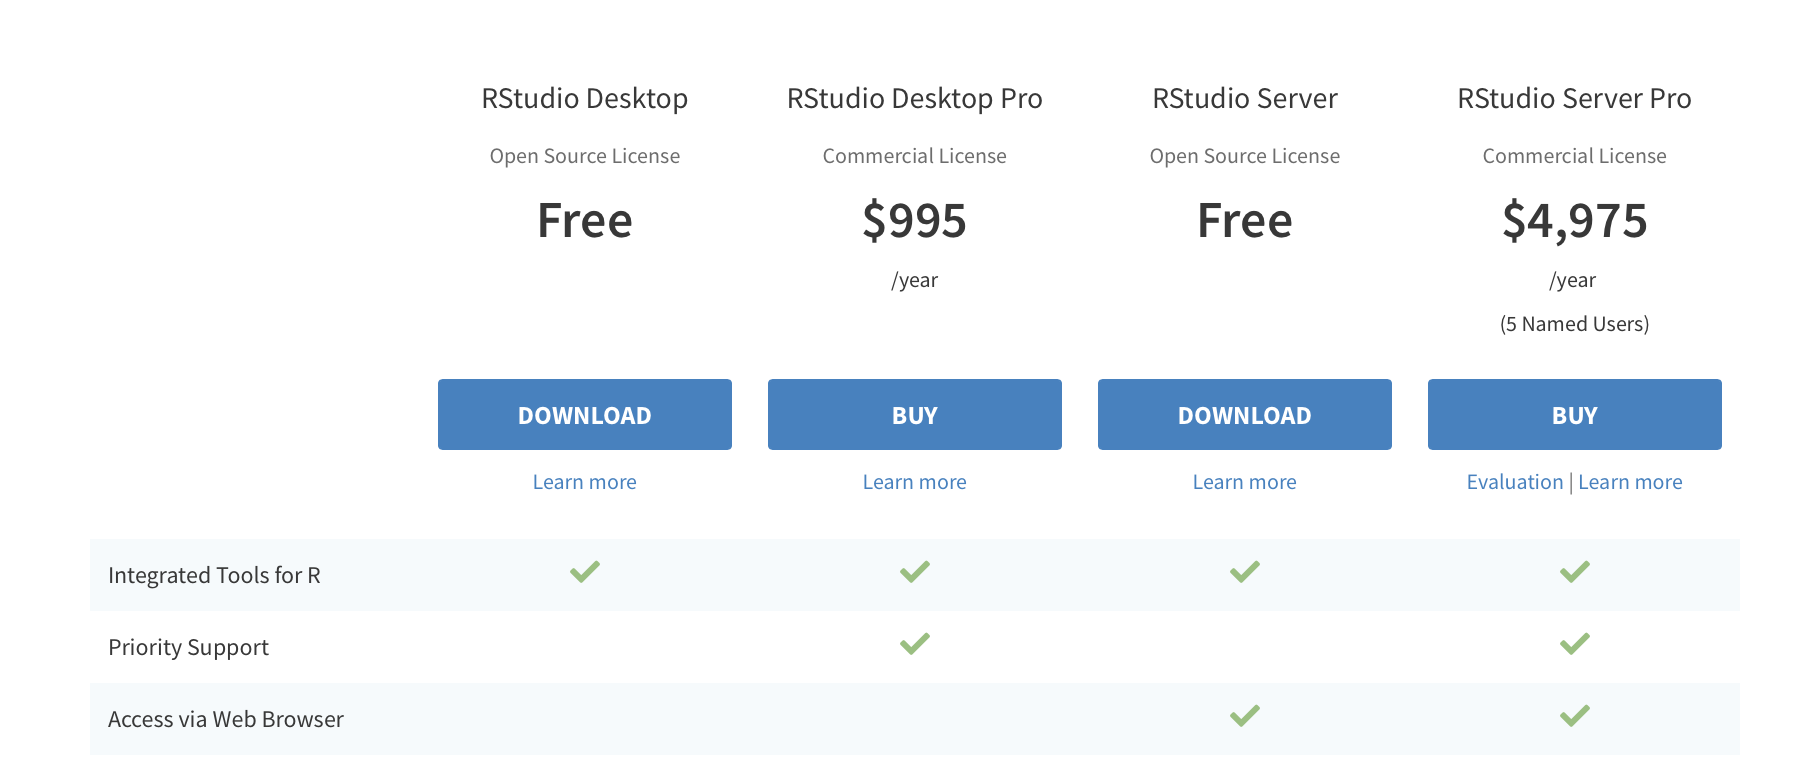
\includegraphics[width=0.8\linewidth]{/home/runner/work/theory_and_practice_of_field_experiments/theory_and_practice_of_field_experiments/Book/Images/new_rstudio} \caption{Select Download in the "RStudio Desktop Open Source License" column.}\label{fig:rstudiopng}
\end{figure}

\begin{figure}
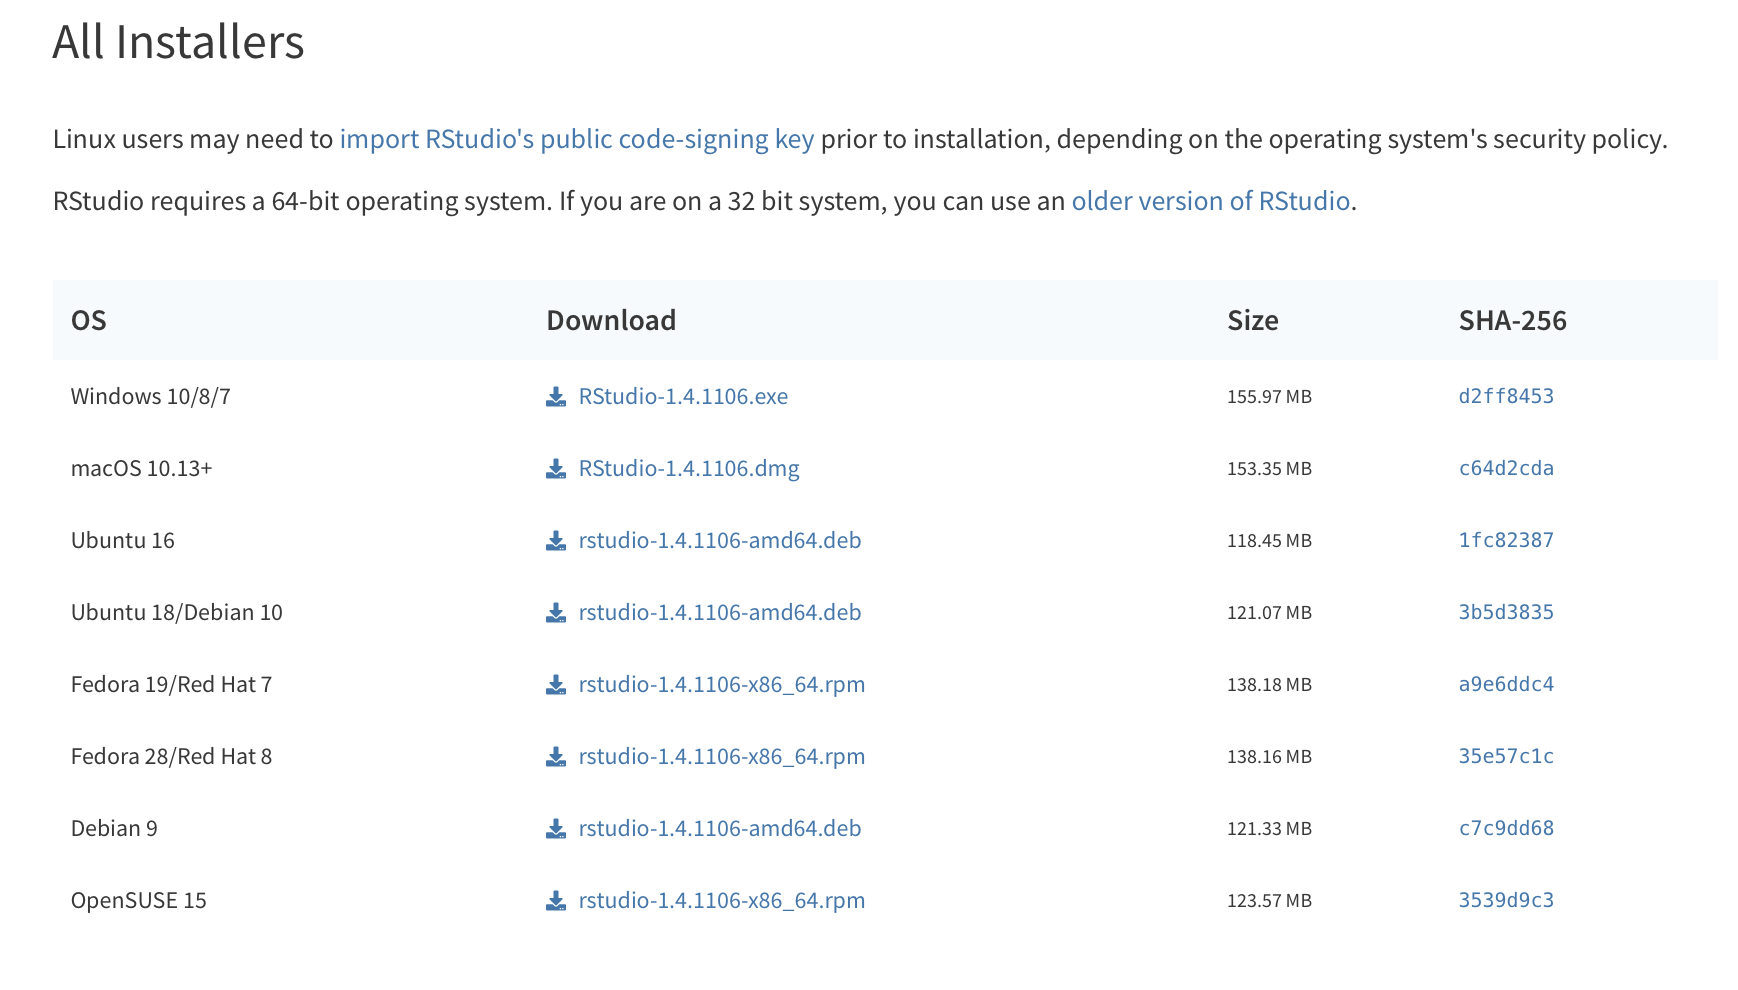
\includegraphics[width=0.8\linewidth]{Images/rstudio_download} \caption{Select the Windows 10/8/7 link for Windows or the Mac OS X 10.13+ link for Mac.}\label{fig:rstudiodownload}
\end{figure}

\hypertarget{rstudio-interface}{%
\section{RStudio Interface}\label{rstudio-interface}}

When you open RStudio for the first time, there should be three panels visible, as depicted in Figure B.3 below.

\begin{itemize}
\tightlist
\item
  Console (left panel)
\item
  Accounting (upper right panel): includes Environment and History tabs
\item
  Miscellaneous (lower right panel)
\end{itemize}

\begin{figure}
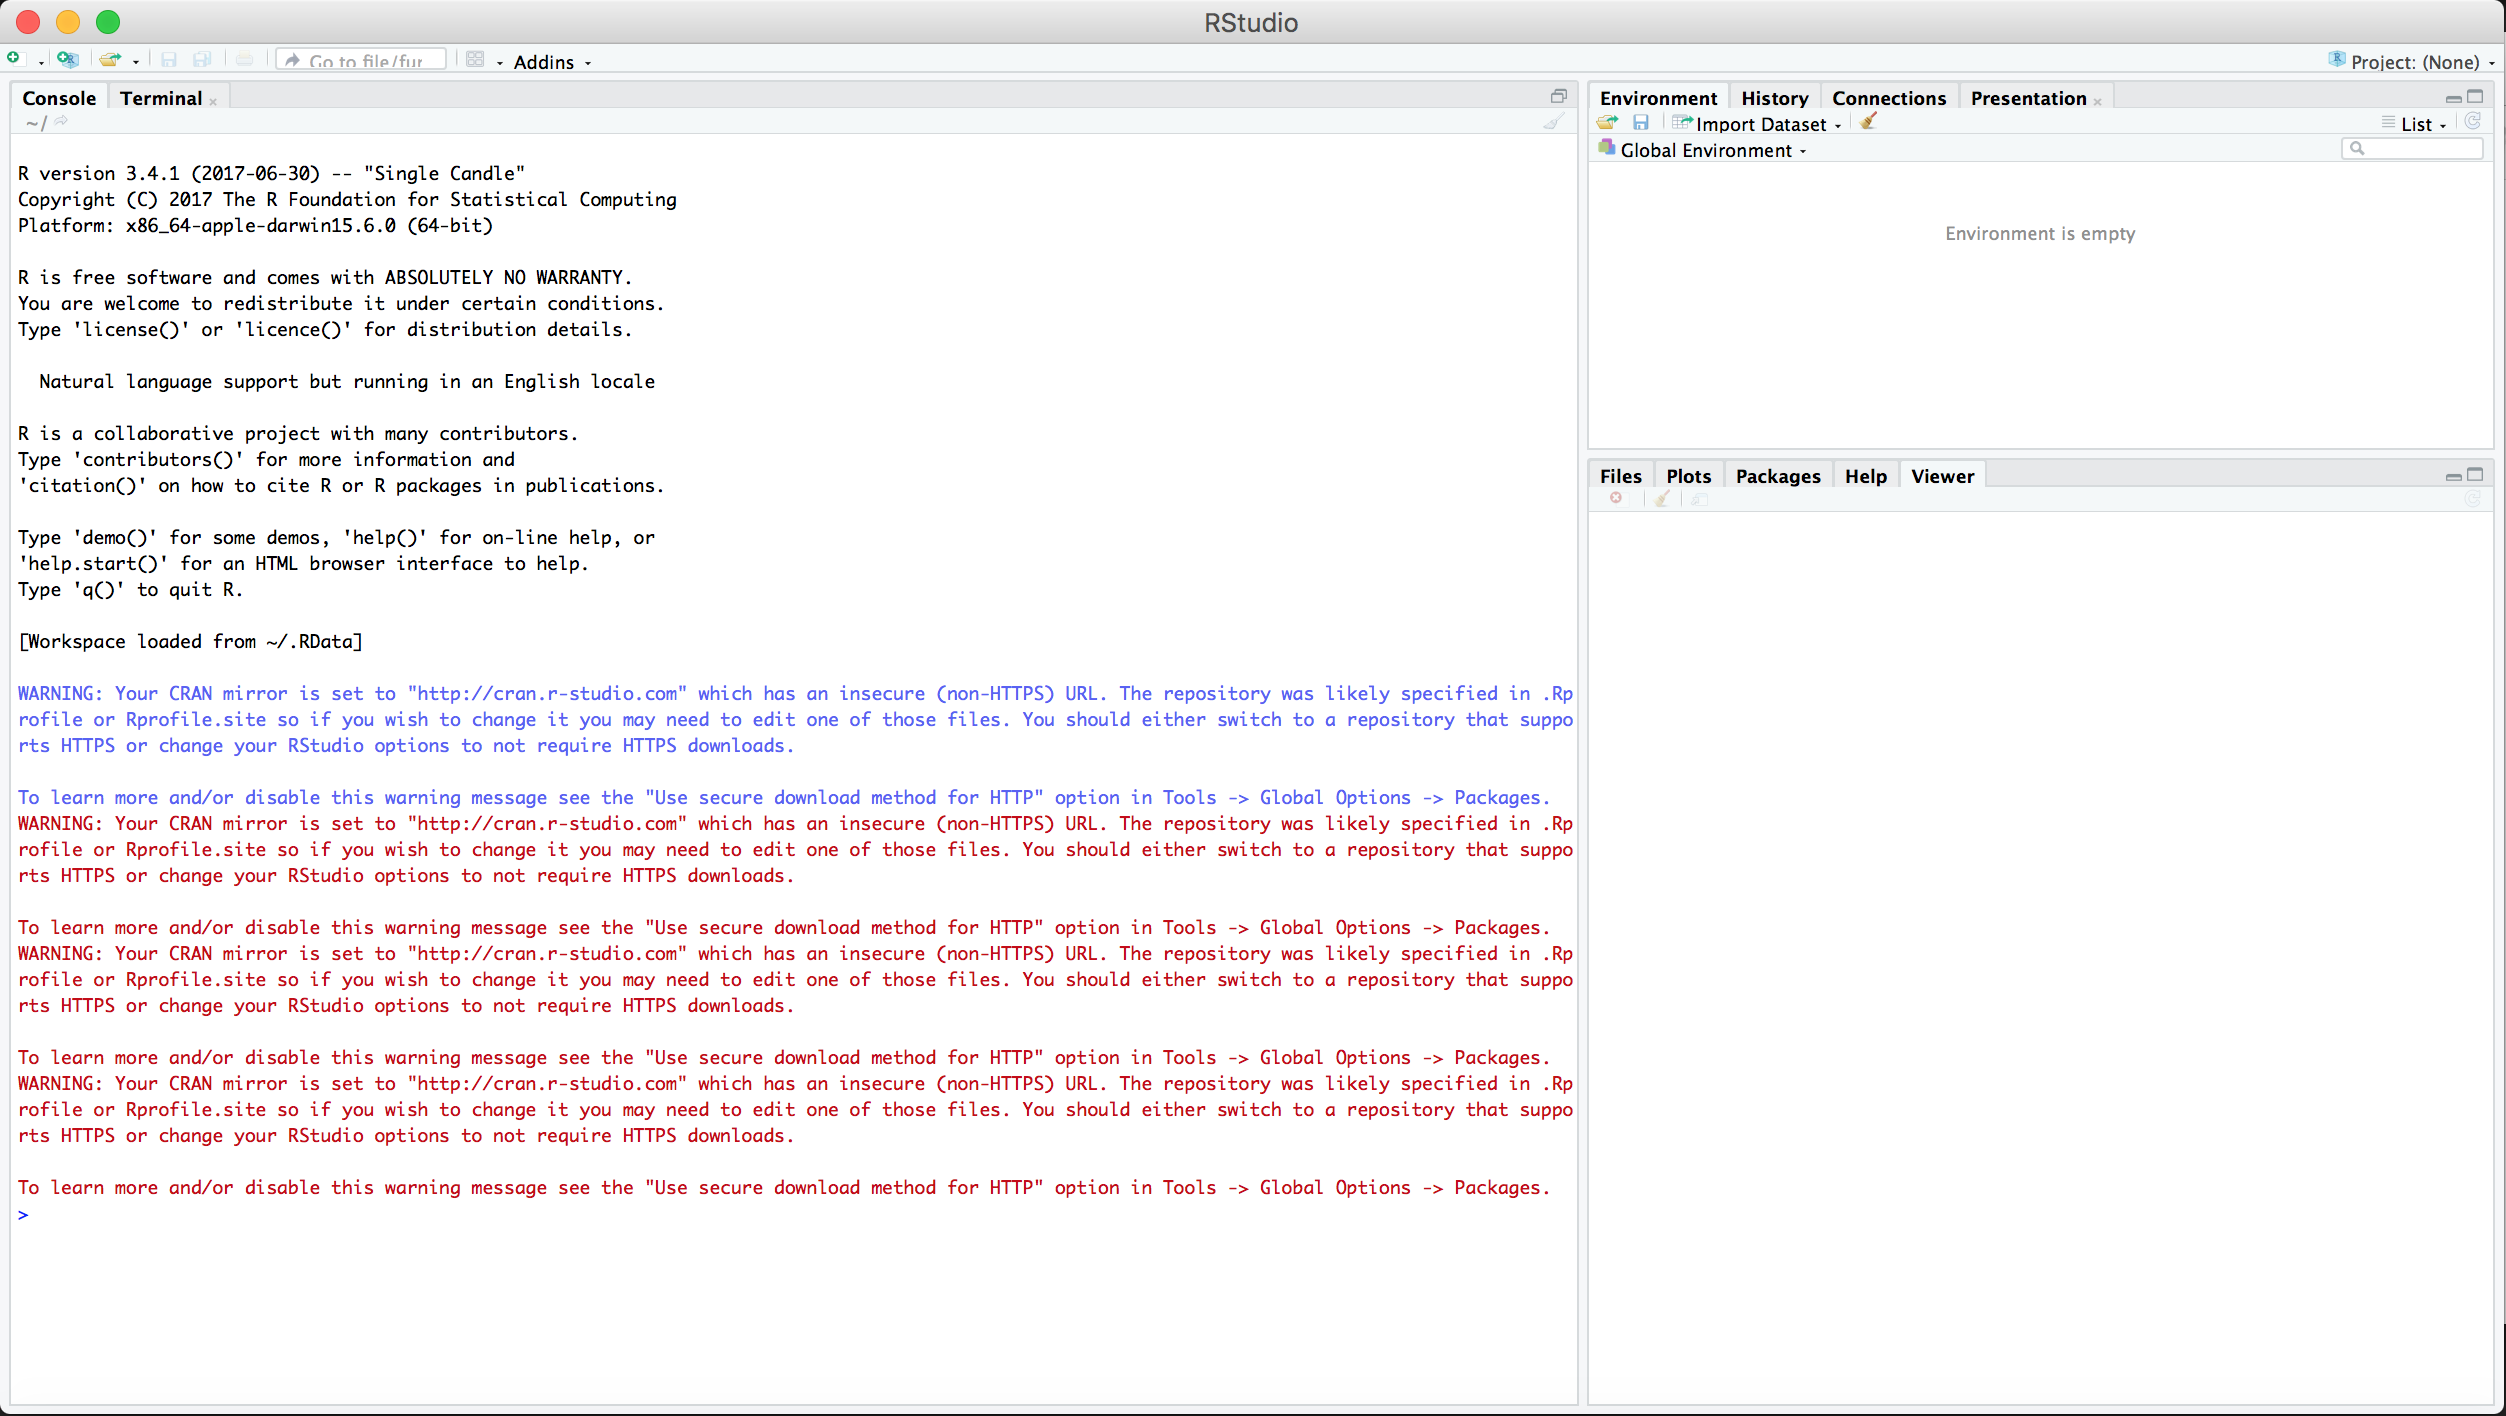
\includegraphics[width=0.8\linewidth]{Images/rstudio_intro} \caption{When you open RStudio, there are three panels visible: the Console (left), Accounting (upper right), and Miscellaneous (lower right).}\label{fig:rstudiointro}
\end{figure}

\hypertarget{console}{%
\subsection{Console}\label{console}}

You can execute all operations in the console. For example if you enter \texttt{4\ +\ 4} and hit the Enter/Return key, the Console will return \texttt{{[}1{]}\ 8}.

To make sure everyone is prepared to use R at Learning Days, we ask participants to run one line of code in the Console to download several R packages. Packages are fragments of reproducible code that allow for more efficient analysis in R. To run these lines, copy the following code into the Console and hit your \texttt{Return}/\texttt{Enter} key. You must be connected to the internet to download packages.

\begin{Shaded}
\begin{Highlighting}[]
\KeywordTok{install.packages}\NormalTok{(}\KeywordTok{c}\NormalTok{(}\StringTok{"ggplot2"}\NormalTok{, }\StringTok{"dplyr"}\NormalTok{, }\StringTok{"AER"}\NormalTok{, }\StringTok{"arm"}\NormalTok{, }\StringTok{"MASS"}\NormalTok{, }\StringTok{"sandwich"}\NormalTok{, }
                   \StringTok{"lmtest"}\NormalTok{, }\StringTok{"estimatr"}\NormalTok{,}\StringTok{"coin"}\NormalTok{,}\StringTok{"randomizr"}\NormalTok{, }\StringTok{"DeclareDesign"}\NormalTok{))}
\end{Highlighting}
\end{Shaded}

If successfully downloaded, your Console will resemble Figure B.4, except that the urls will differ depending on your location.

\begin{figure}
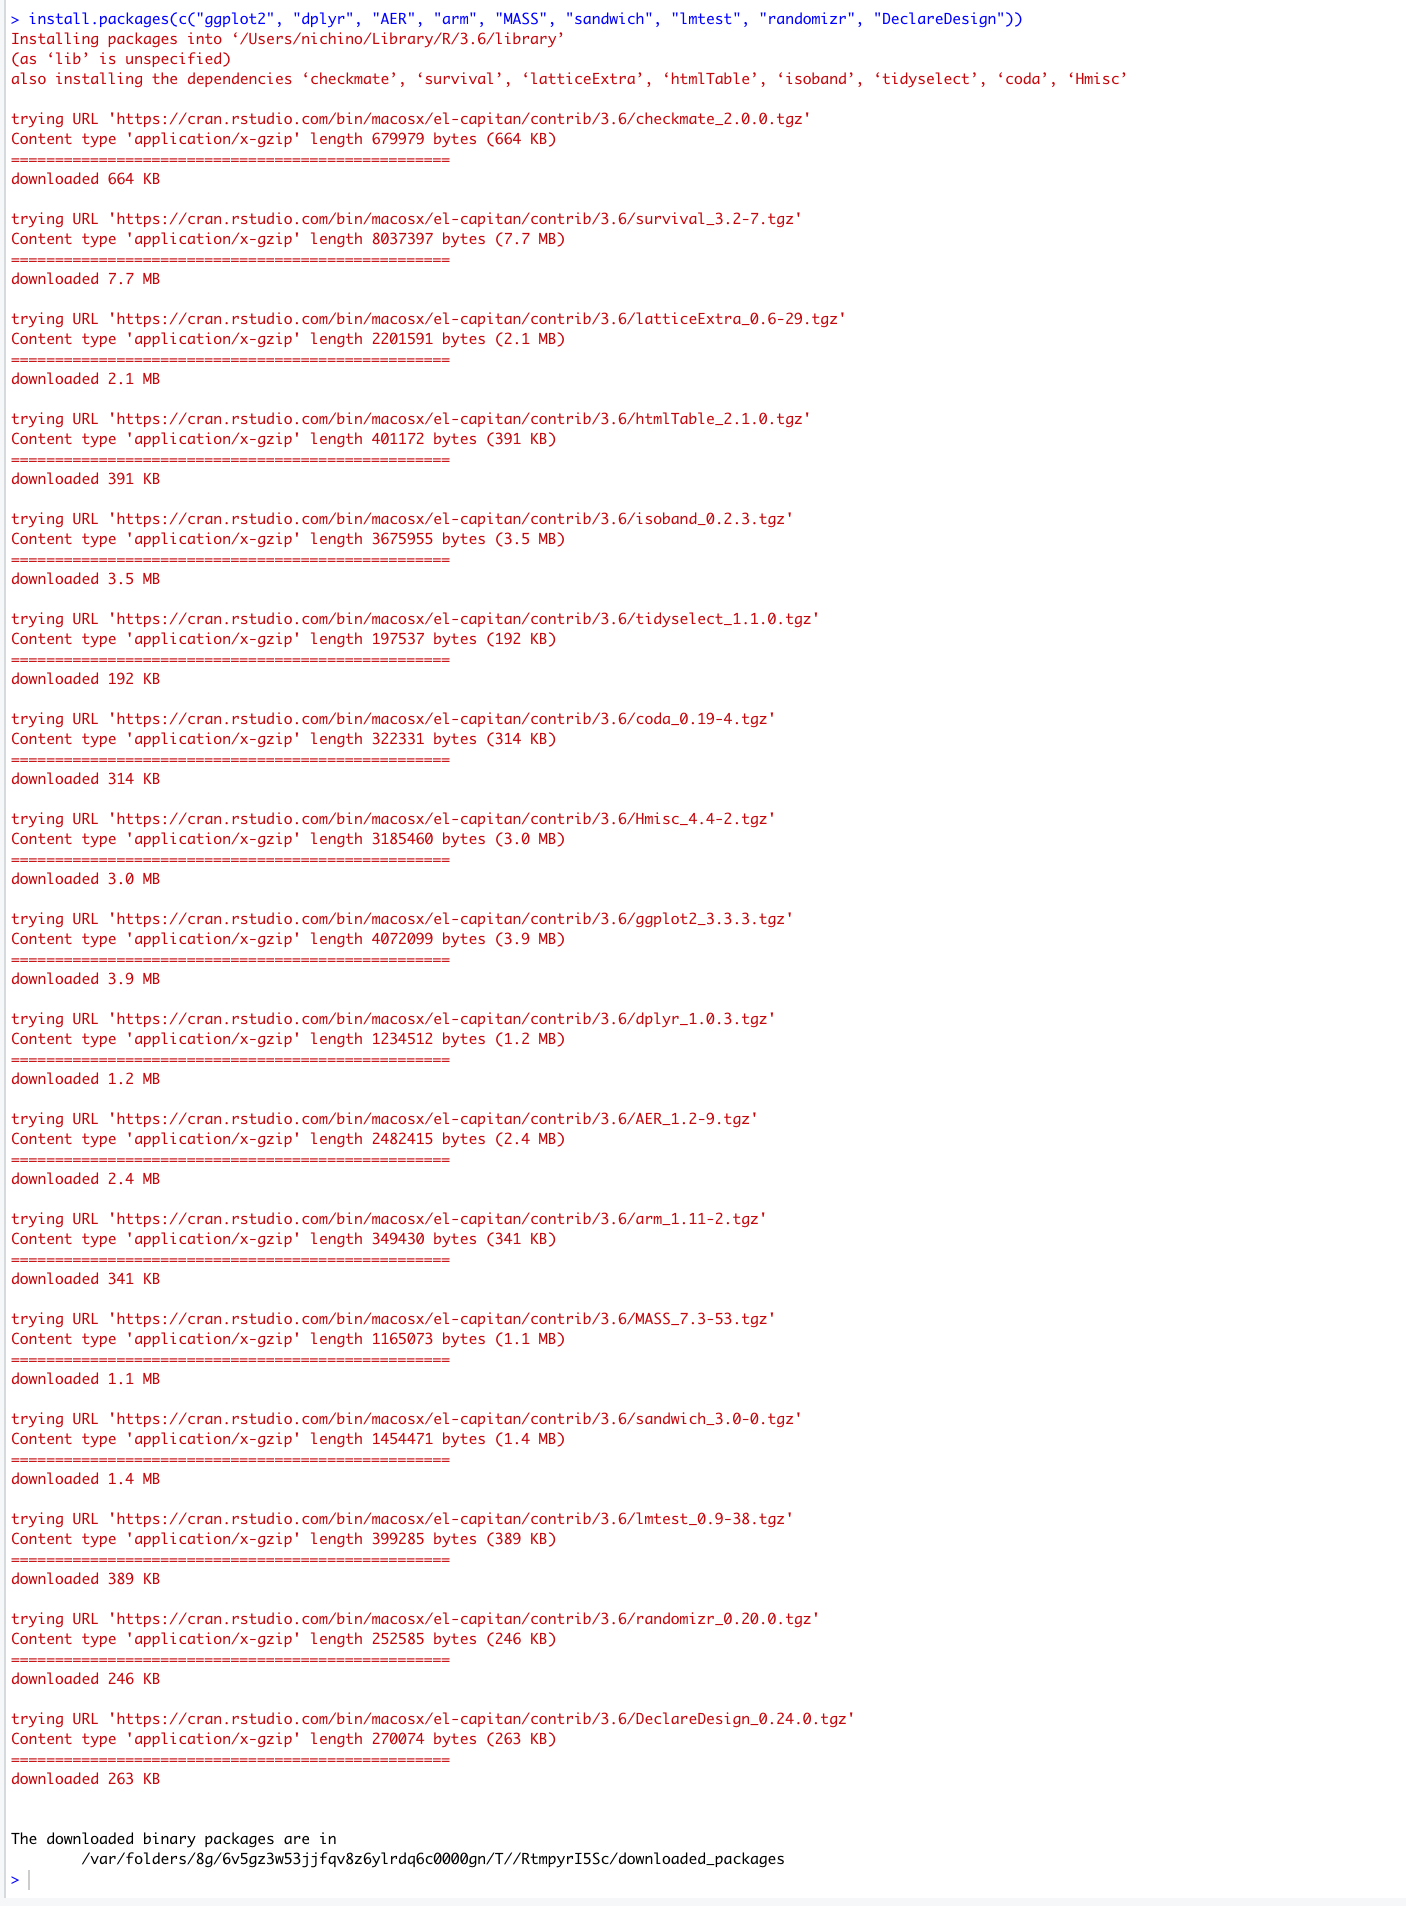
\includegraphics[width=0.4\linewidth]{Images/console2a} \caption{An image of the Console after executing the three lines of code listed above.}\label{fig:console2}
\end{figure}

\hypertarget{editor}{%
\subsection{Editor}\label{editor}}

In order to write and save reproducible code, we will open a fourth panel, the Editor, by clicking on the icon with a white page with a plus sign on the upper-left corner of the RStudio interface and selecting \texttt{R\ Script}, as depicted in Figure B.5.

\begin{figure}
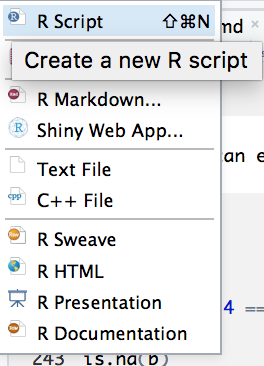
\includegraphics[width=0.6\linewidth]{Images/new_script} \caption{Create a new R script and open the editor panel by selecting `R Script` from the dropdown menu.}\label{fig:newscript}
\end{figure}

Once the R script is opened, there should be four panels within the RStudio interface, now with the addition of the Editor panel. We can execute simple arithmetic by entering a formula in the editor and pressing \texttt{Control\ +\ Enter} (Windows) or \texttt{Command\ +\ Enter} (Mac). The formula and the ``answer'' will appear in the Console, as depicted in Figure B.6, with red boxes added for emphasis.

\begin{figure}
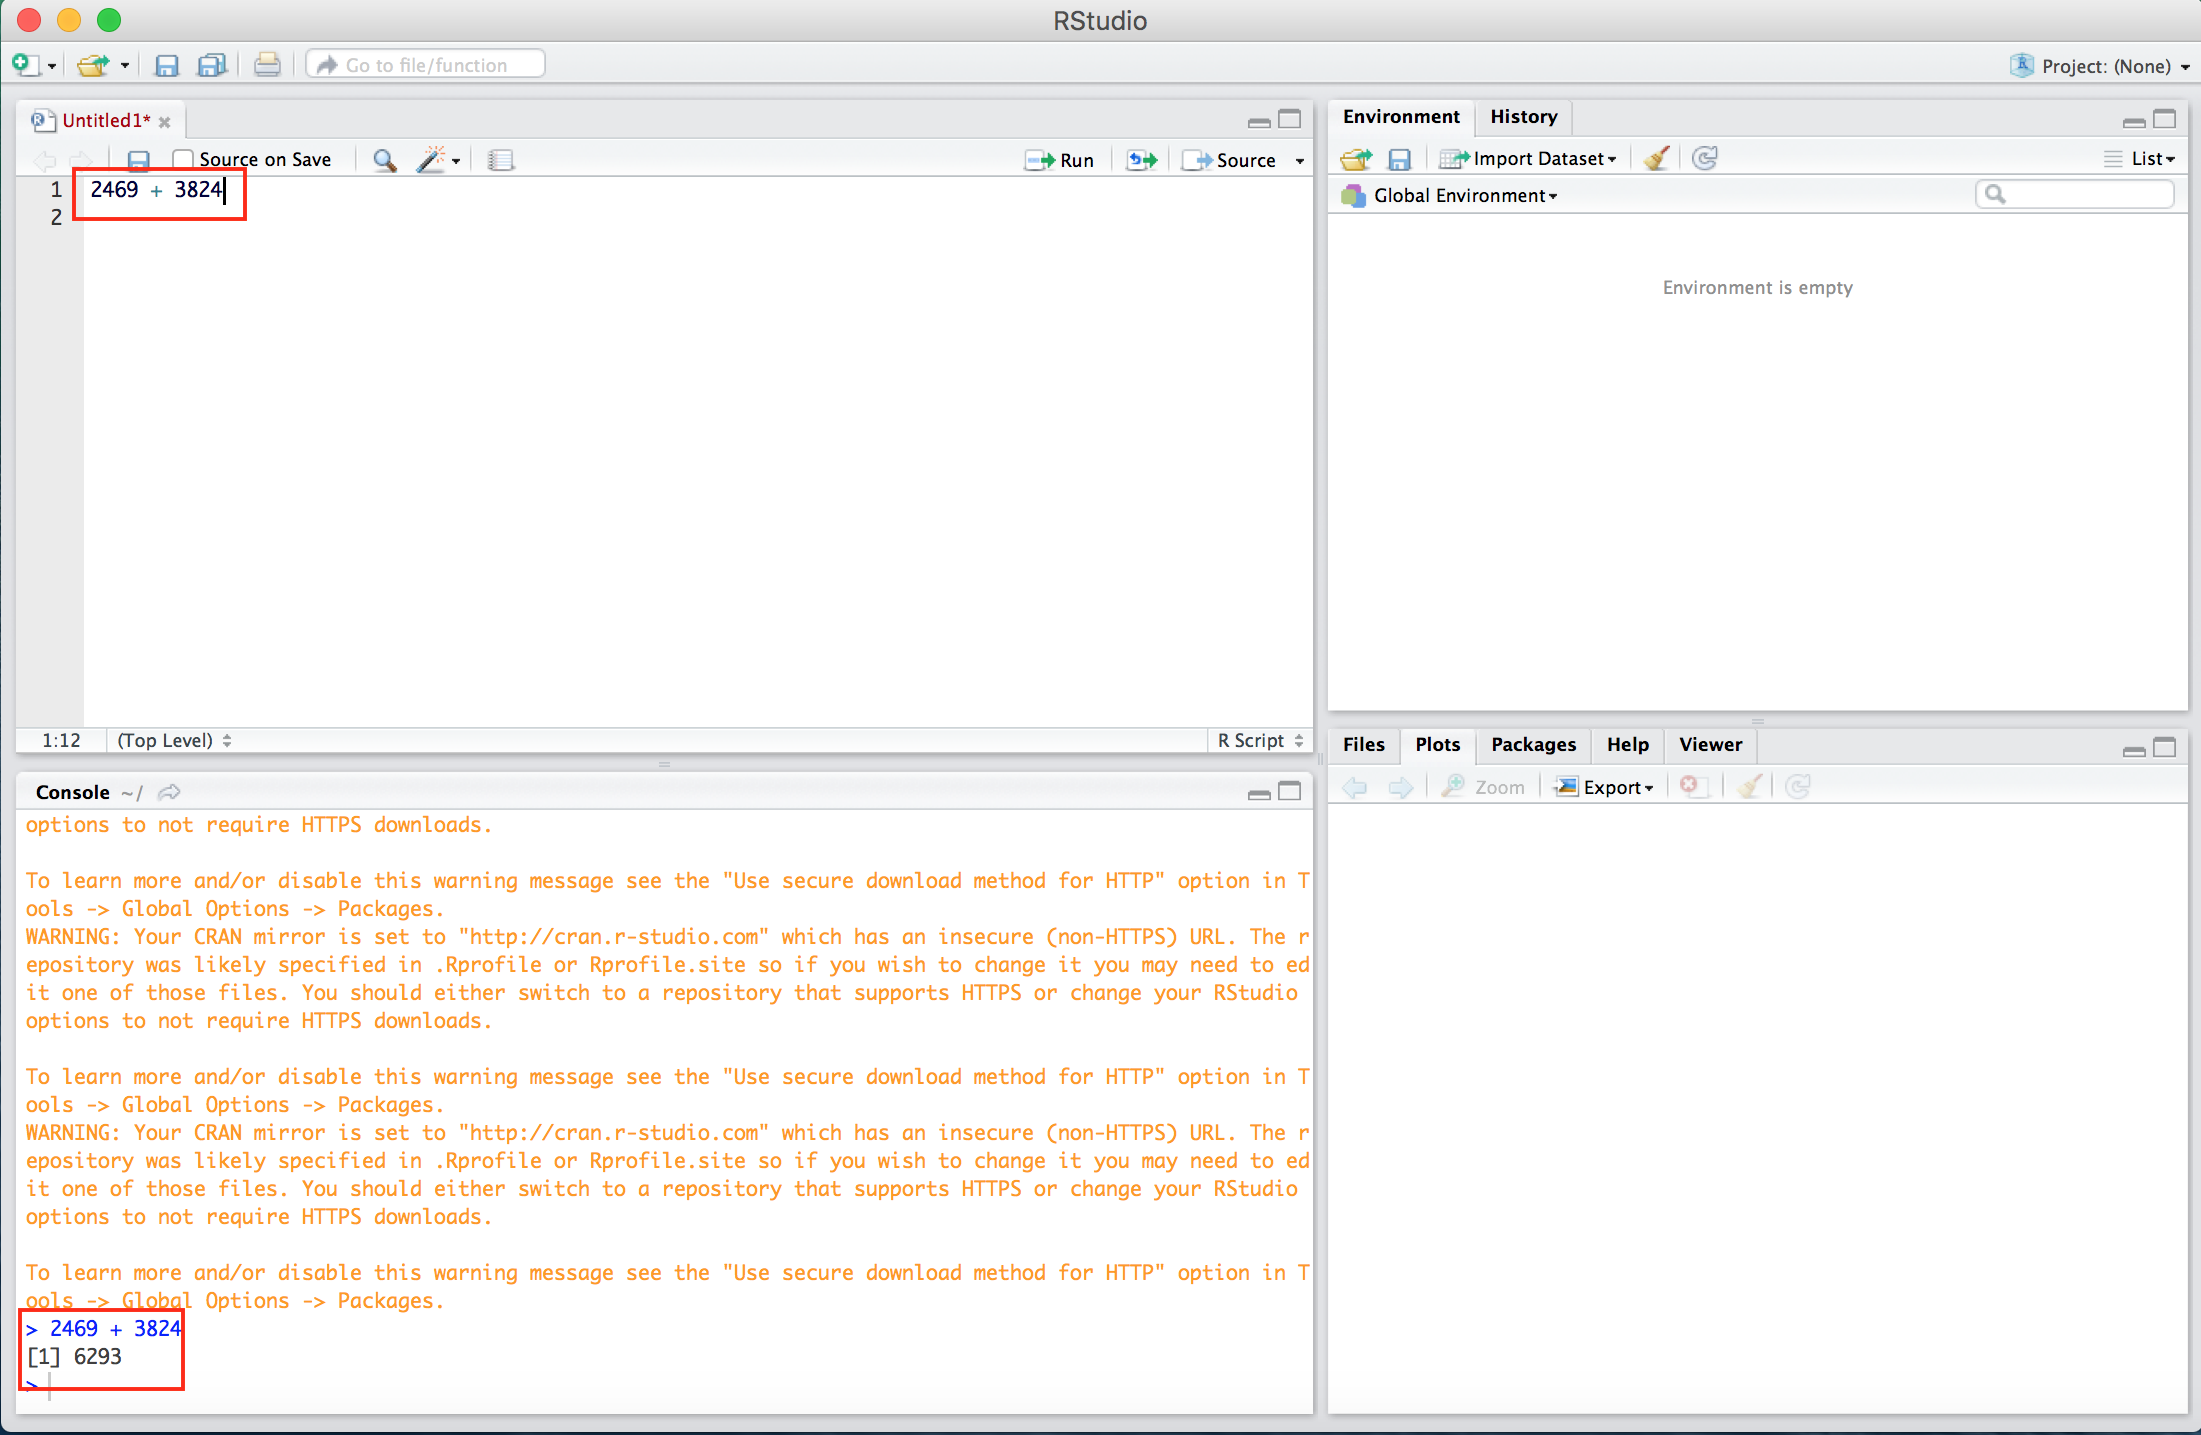
\includegraphics[width=0.6\linewidth]{Images/first_addition} \caption{An arithmetic expression is entered in the editor and evaluated in the console. The red boxes are added for emphasis.}\label{fig:firstaddition}
\end{figure}

R can be used for any arithmetic operation including, but not limited to, addition (\texttt{+}), subtraction (\texttt{-}), scalar multiplication (\texttt{*}), division (\texttt{/}), and exponentiation (\texttt{\^{}}).

\hypertarget{accounting}{%
\subsection{Accounting}\label{accounting}}

Beyond basic functions, we can also store values, data, and functions in the global environment. To assign a value to a variable, use the \texttt{\textless{}-} operator. All stored values, functions, and data will appear in the Environment tab in the Accounting panel. In Figure B.7, we define the variable \texttt{t} to take the value \(3 \times \frac{6}{14}\), and can see that it is stored under Values.

We also load a dataset. Here, ``ChickWeight'' is a dataset built into R; most datasets will be loaded from the web or other files on your computer through an alternate method. We can see that ChickWeight contains 578 observations of 4 variables and is stored in the Environment. By clicking on the name ChickWeight a tab will enter with the dataset in your Editor window.

\begin{figure}
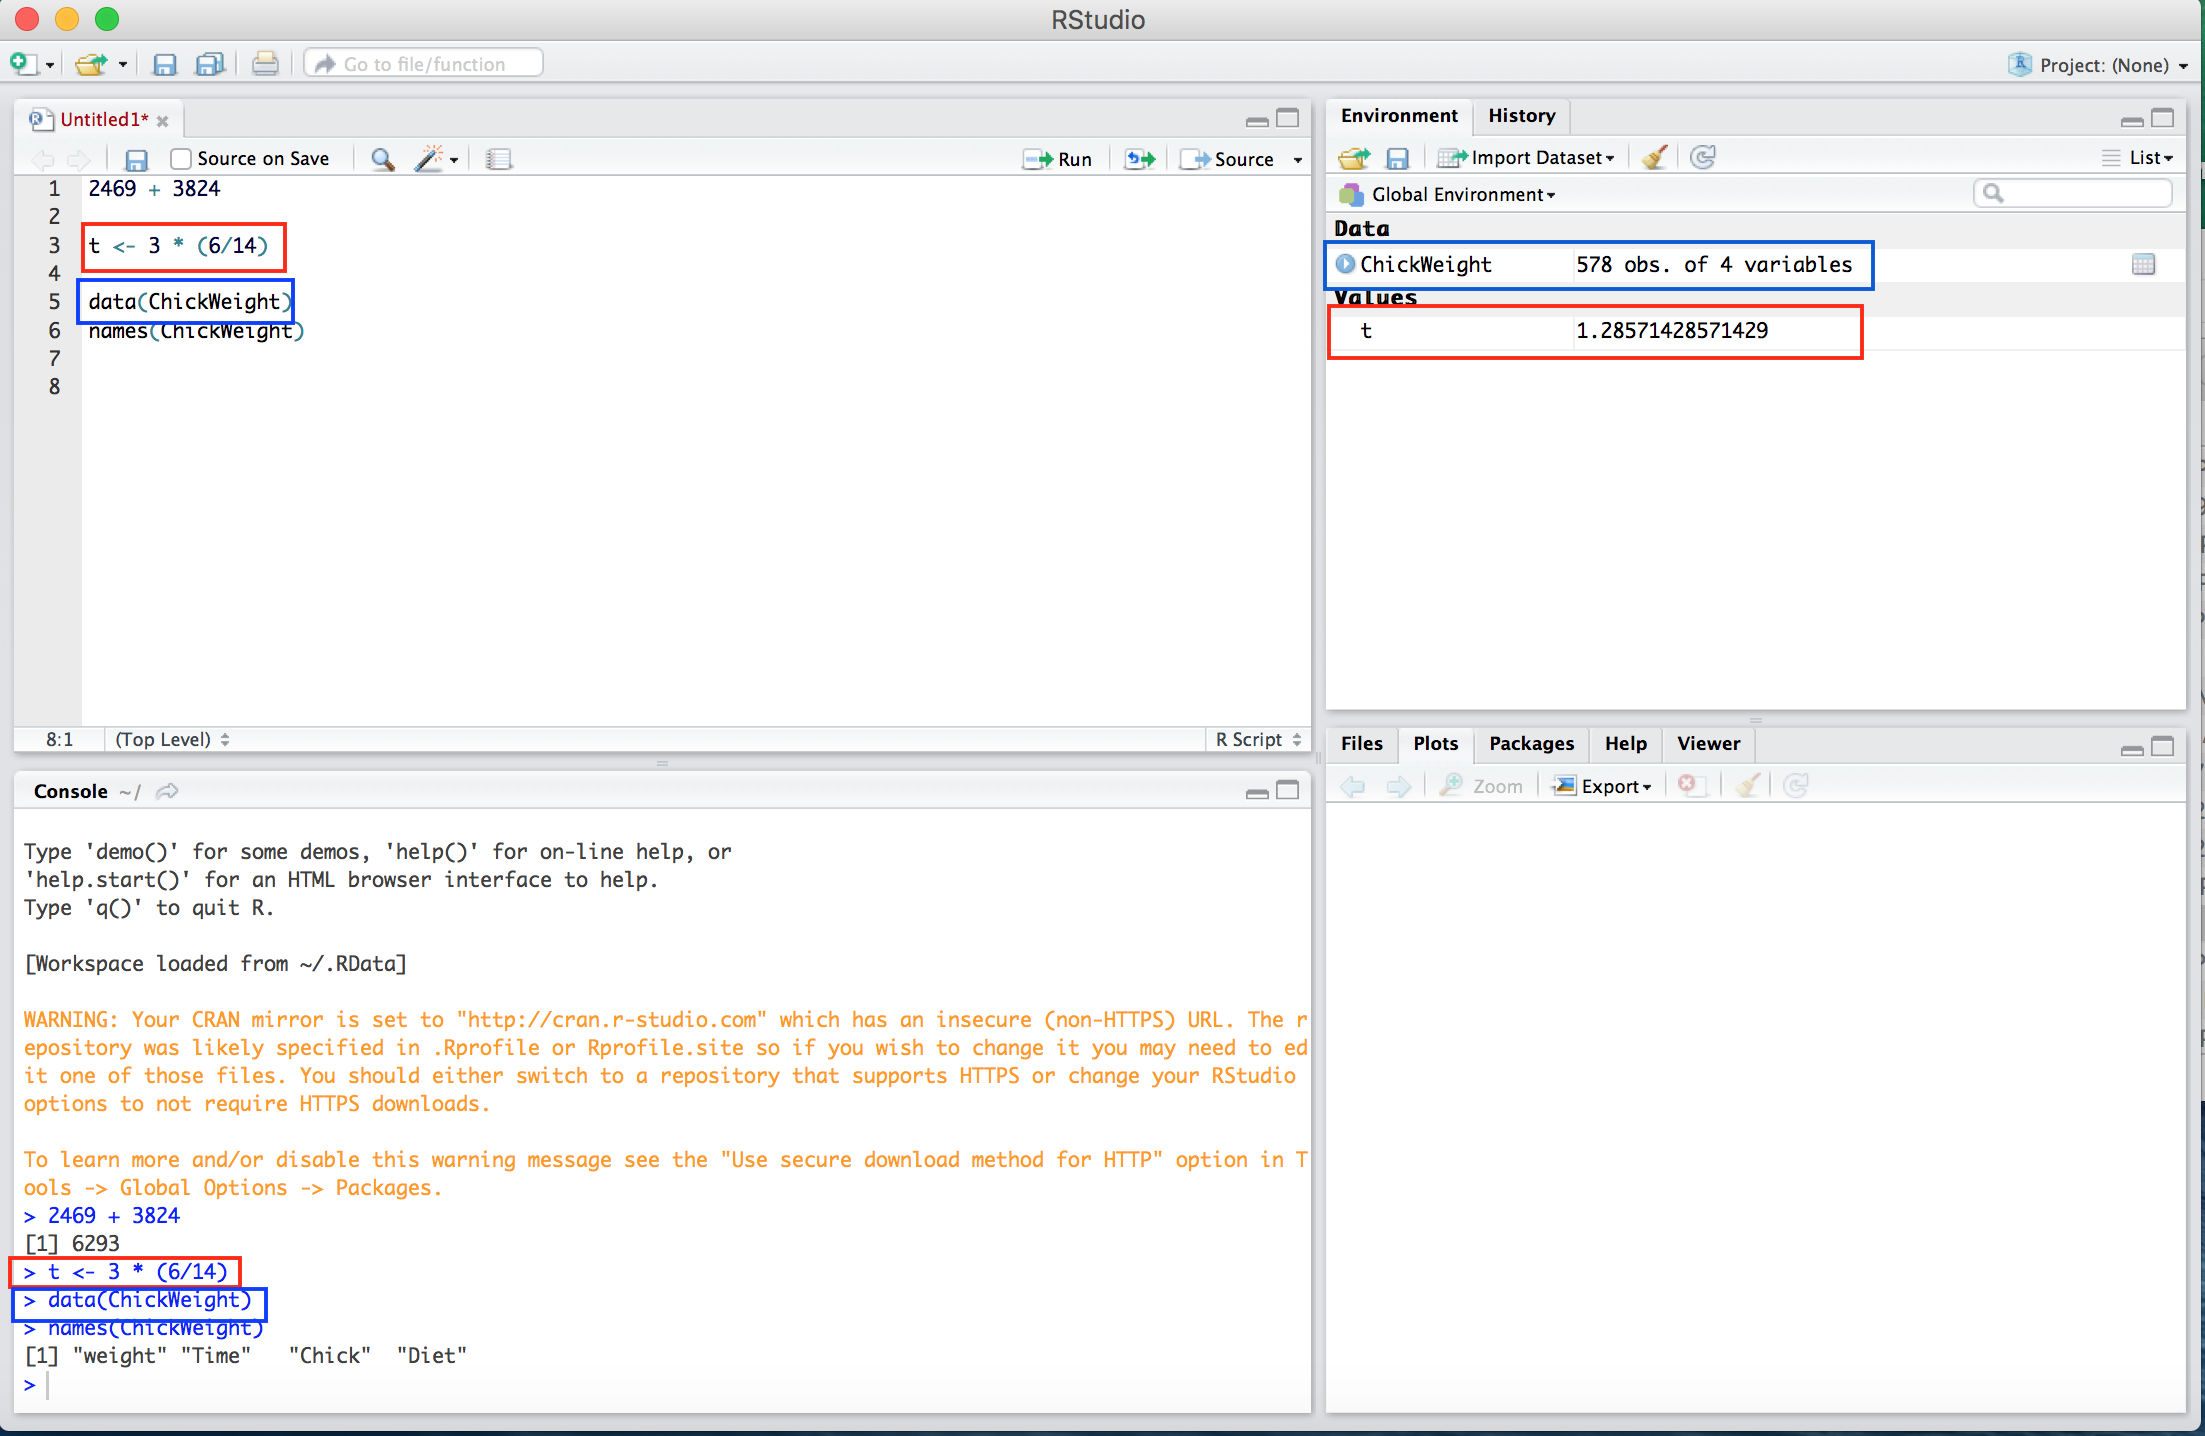
\includegraphics[width=0.6\linewidth]{Images/save_data} \caption{The value 3 * (6/14) is assigned to the variable t (red) and the dataset ChickWeight is added to the global environment (blue). The boxes are added for emphasis.}\label{fig:savedata}
\end{figure}

The Learning Days workshops use many tools in R to analyze and view data. For now, we can learn some basic tools to examine the data. The function \texttt{head()} allows us to see the first six rows of the dataset. \texttt{summary()} summarizes each of the columns of the dataset and \texttt{dim()} provides the dimensions of the dataset with first the number of rows and then columns.

\begin{Shaded}
\begin{Highlighting}[]
\KeywordTok{head}\NormalTok{(ChickWeight) }\CommentTok{# First 6 observations in dataset}
\end{Highlighting}
\end{Shaded}

\begin{verbatim}
  weight Time Chick Diet
1     42    0     1    1
2     51    2     1    1
3     59    4     1    1
4     64    6     1    1
5     76    8     1    1
6     93   10     1    1
\end{verbatim}

\begin{Shaded}
\begin{Highlighting}[]
\KeywordTok{summary}\NormalTok{(ChickWeight) }\CommentTok{# Summary of all variables}
\end{Highlighting}
\end{Shaded}

\begin{verbatim}
     weight         Time          Chick     Diet   
 Min.   : 35   Min.   : 0.0   13     : 12   1:220  
 1st Qu.: 63   1st Qu.: 4.0   9      : 12   2:120  
 Median :103   Median :10.0   20     : 12   3:120  
 Mean   :122   Mean   :10.7   10     : 12   4:118  
 3rd Qu.:164   3rd Qu.:16.0   17     : 12          
 Max.   :373   Max.   :21.0   19     : 12          
                              (Other):506          
\end{verbatim}

\begin{Shaded}
\begin{Highlighting}[]
\KeywordTok{dim}\NormalTok{(ChickWeight) }\CommentTok{# Dimensions of the dataset in the order rows, columns}
\end{Highlighting}
\end{Shaded}

\begin{verbatim}
[1] 578   4
\end{verbatim}

Unlike other statistical software, R allows users to store multiple datasets, possibly of different dimensions, simultaneously. This feature makes R quite flexible for analysis using multiple methods.

\hypertarget{miscellaneous}{%
\subsection{Miscellaneous}\label{miscellaneous}}

R provides a suite of tools, ranging from built-in plot functions to packages to graph data, models, estimates, etc. The final Miscellaneous panel allows for the quick viewing of graphs in RStudio. Figure B.8 shows a plot in this panel. Leaning Days will discuss how to plot data; for now, don't worry about the graphing the code in the Editor.

\begin{figure}
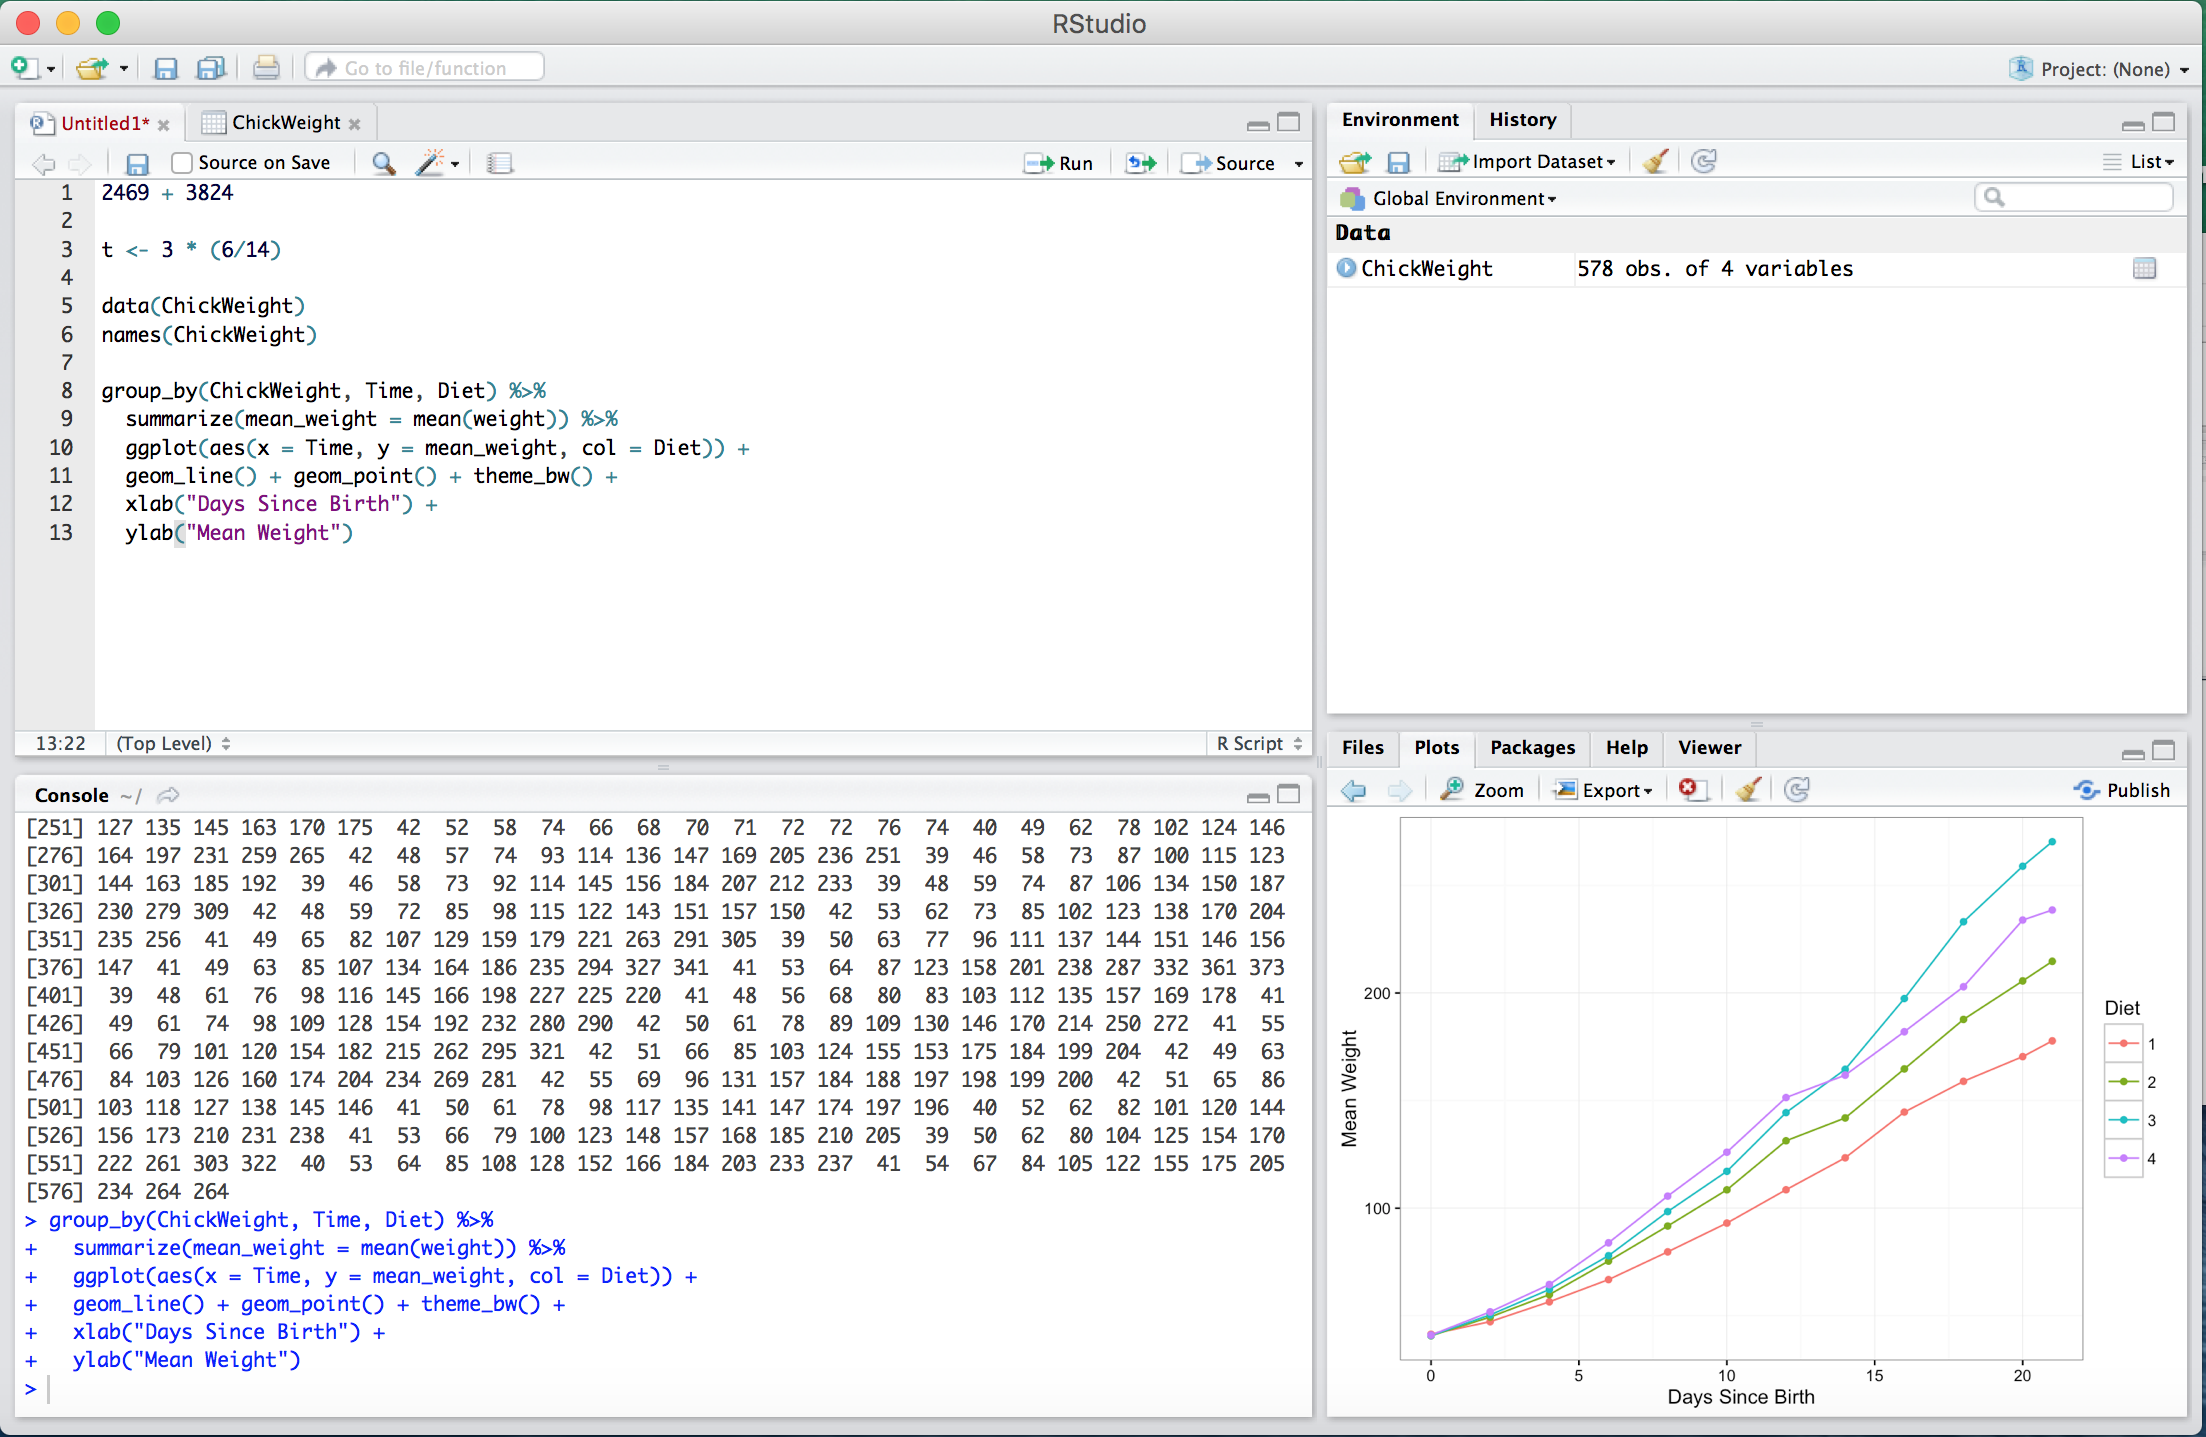
\includegraphics[width=0.6\linewidth]{Images/graph} \caption{An example plot of the `ChickWeight` data made in R.}\label{fig:graph}
\end{figure}

\hypertarget{learning-to-use-r}{%
\section{Learning to Use R}\label{learning-to-use-r}}

\hypertarget{online-resources}{%
\subsection{Online Resources}\label{online-resources}}

There are many helpful online resources to help you start learning R. We recommend two sources:

\begin{itemize}
\tightlist
\item
  Code School, which runs entirely through your browser \url{https://www.codeschool.com/courses/try-r}.
\item
  Coursera, via an online R Programming course organized by Johns Hopkins University:

  \begin{enumerate}
  \def\labelenumi{\roman{enumi}.}
  \tightlist
  \item
    Go to \url{https://www.coursera.org}
  \item
    Create an account (this is free!)
  \item
    Sign up for R Programming at Johns Hopkins University (instructor: Roger Peng) under the ``Courses'' tab
  \item
    Read the materials and watch the videos from the first week. The videos from the first week are about 2.5 hours long total.
  \end{enumerate}
\end{itemize}

\hypertarget{basic-practice}{%
\subsection{Basic Practice}\label{basic-practice}}

Here we provide some fragments of code to familiarize you with some basic practices in R. We recommend that you practice by typing the code fragments into your Editor and then evaluating them.

\hypertarget{setting-up-an-r-session}{%
\subsubsection{Setting up an R Session}\label{setting-up-an-r-session}}

In general, we read other files such as data or functions into R and output results like graphs or tables into files not contained within an R session. To do this, we must give R an ``address'' at which it can locate such files. It may be most efficient to do this by setting a working directory, a file path at which relevant files are stored. We can identify the current working directory using \texttt{getwd()} and set a new one using \texttt{setwd()}. Note that the syntax of these filepaths varies by operating system.

\begin{Shaded}
\begin{Highlighting}[]
\KeywordTok{getwd}\NormalTok{()}
\end{Highlighting}
\end{Shaded}

\begin{Shaded}
\begin{Highlighting}[]
\KeywordTok{setwd}\NormalTok{(}\StringTok{"~TaraLyn/EGAP Learning Days Admin/Workshop 2018_2 (Uruguay)/"}\NormalTok{)   }
\end{Highlighting}
\end{Shaded}

You may need to install packages beyond those listed above to execute certain functions. To install packages we use \texttt{install.packages("")}, filling in the package name between the "" marks, as follows. You need only install packages once.

\begin{Shaded}
\begin{Highlighting}[]
\KeywordTok{install.packages}\NormalTok{(}\StringTok{"randomizr"}\NormalTok{)  }
\end{Highlighting}
\end{Shaded}

Once a package is installed, it can be loaded and accessed using \texttt{library()} where the package name is inserted between the parentheses (no "" marks).

\begin{Shaded}
\begin{Highlighting}[]
\KeywordTok{library}\NormalTok{(randomizr)}
\end{Highlighting}
\end{Shaded}

To clear R's memory of the stored data, functions, or values that appear in the accounting tab, use \texttt{rm(list\ =\ ls())}. It may be useful to set a random number seed to ensure that replication is possible in a different R session, particularly when we work with simulation-based methods.

\begin{Shaded}
\begin{Highlighting}[]
\KeywordTok{rm}\NormalTok{(}\DataTypeTok{list =} \KeywordTok{ls}\NormalTok{())                                   }
\KeywordTok{set.seed}\NormalTok{(}\DecValTok{2018}\NormalTok{)  }\CommentTok{# Optional: Set a seed to make output replicable}
\end{Highlighting}
\end{Shaded}

\hypertarget{r-basics}{%
\subsubsection{R Basics}\label{r-basics}}

We now explore some basic commands. In order to assign a scalar (single element) to a variable, we use the \texttt{\textless{}-} command as discussed previously:

\begin{Shaded}
\begin{Highlighting}[]
\CommentTok{# "<-"  is the assignment command; it is used to define things. eg:}
\NormalTok{(a <-}\StringTok{ }\DecValTok{5}\NormalTok{)     }
\end{Highlighting}
\end{Shaded}

\begin{verbatim}
[1] 5
\end{verbatim}

We may also want to assign a vector of elements to a variable. Here we use the same \texttt{\textless{}-} command, but focus on how to create the vector.

\begin{Shaded}
\begin{Highlighting}[]
\NormalTok{(b <-}\StringTok{ }\DecValTok{1}\OperatorTok{:}\DecValTok{10}\NormalTok{)              }\CommentTok{# ":"  is used to define a string of integers}
\end{Highlighting}
\end{Shaded}

\begin{verbatim}
 [1]  1  2  3  4  5  6  7  8  9 10
\end{verbatim}

\begin{Shaded}
\begin{Highlighting}[]
\NormalTok{(v <-}\StringTok{ }\KeywordTok{c}\NormalTok{(}\DecValTok{1}\NormalTok{, }\DecValTok{3}\NormalTok{, }\DecValTok{2}\NormalTok{, }\DecValTok{4}\NormalTok{, pi))   }\CommentTok{# use c() to make a vector with anything in it}
\end{Highlighting}
\end{Shaded}

\begin{verbatim}
[1] 1.000 3.000 2.000 4.000 3.142
\end{verbatim}

We can then refer to elements of a vector by denoting their position in a vector inside hard brackets \texttt{{[}{]}}.

\begin{Shaded}
\begin{Highlighting}[]
\CommentTok{# Extract elements of a vector:}
\NormalTok{b[}\DecValTok{1}\NormalTok{]                   }\CommentTok{# Returns position 1}
\end{Highlighting}
\end{Shaded}

\begin{verbatim}
[1] 1
\end{verbatim}

\begin{Shaded}
\begin{Highlighting}[]
\NormalTok{b[}\DecValTok{5}\OperatorTok{:}\DecValTok{4}\NormalTok{]                 }\CommentTok{# Returns positions 5 and 4, in that order}
\end{Highlighting}
\end{Shaded}

\begin{verbatim}
[1] 5 4
\end{verbatim}

\begin{Shaded}
\begin{Highlighting}[]
\NormalTok{b[}\OperatorTok{-}\DecValTok{1}\NormalTok{]                  }\CommentTok{# Returns all but the first number  }
\end{Highlighting}
\end{Shaded}

\begin{verbatim}
[1]  2  3  4  5  6  7  8  9 10
\end{verbatim}

\begin{Shaded}
\begin{Highlighting}[]
\CommentTok{# Returns all numbers indicated as "TRUE"}
\NormalTok{b[}\KeywordTok{c}\NormalTok{(}\OtherTok{TRUE}\NormalTok{, }\OtherTok{FALSE}\NormalTok{, }\OtherTok{TRUE}\NormalTok{, }\OtherTok{FALSE}\NormalTok{, }\OtherTok{FALSE}\NormalTok{, }\OtherTok{TRUE}\NormalTok{, }\OtherTok{TRUE}\NormalTok{, }\OtherTok{FALSE}\NormalTok{, }\OtherTok{FALSE}\NormalTok{, }\OtherTok{FALSE}\NormalTok{)]  }
\end{Highlighting}
\end{Shaded}

\begin{verbatim}
[1] 1 3 6 7
\end{verbatim}

\begin{Shaded}
\begin{Highlighting}[]
\CommentTok{# Assign new values to particular elements of a vector}
\NormalTok{b[}\DecValTok{5}\NormalTok{] <-}\StringTok{ }\DecValTok{0}
\end{Highlighting}
\end{Shaded}

There are a set of built-in functions that can be applied to vectors like \texttt{b}.

\begin{Shaded}
\begin{Highlighting}[]
\KeywordTok{sum}\NormalTok{(b)      }\CommentTok{# Sum of all elements}
\end{Highlighting}
\end{Shaded}

\begin{verbatim}
[1] 50
\end{verbatim}

\begin{Shaded}
\begin{Highlighting}[]
\KeywordTok{mean}\NormalTok{(b)     }\CommentTok{# Mean of all elements}
\end{Highlighting}
\end{Shaded}

\begin{verbatim}
[1] 5
\end{verbatim}

\begin{Shaded}
\begin{Highlighting}[]
\KeywordTok{max}\NormalTok{(b)      }\CommentTok{# Maximum of all elements}
\end{Highlighting}
\end{Shaded}

\begin{verbatim}
[1] 10
\end{verbatim}

\begin{Shaded}
\begin{Highlighting}[]
\KeywordTok{min}\NormalTok{(b)      }\CommentTok{# Minimum of all elements}
\end{Highlighting}
\end{Shaded}

\begin{verbatim}
[1] 0
\end{verbatim}

\begin{Shaded}
\begin{Highlighting}[]
\KeywordTok{sd}\NormalTok{(b)       }\CommentTok{# Standard deviation of all elements}
\end{Highlighting}
\end{Shaded}

\begin{verbatim}
[1] 3.496
\end{verbatim}

\begin{Shaded}
\begin{Highlighting}[]
\KeywordTok{var}\NormalTok{(b)      }\CommentTok{# Variance of all elements}
\end{Highlighting}
\end{Shaded}

\begin{verbatim}
[1] 12.22
\end{verbatim}

We can also apply arithmetic transformations to all elements of a vector:

\begin{Shaded}
\begin{Highlighting}[]
\NormalTok{b}\OperatorTok{^}\DecValTok{2}               \CommentTok{# Square the variable}
\end{Highlighting}
\end{Shaded}

\begin{verbatim}
 [1]   1   4   9  16   0  36  49  64  81 100
\end{verbatim}

\begin{Shaded}
\begin{Highlighting}[]
\NormalTok{b}\OperatorTok{^}\NormalTok{.}\DecValTok{5}              \CommentTok{# Square root of the variable}
\end{Highlighting}
\end{Shaded}

\begin{verbatim}
 [1] 1.000 1.414 1.732 2.000 0.000 2.449 2.646 2.828 3.000 3.162
\end{verbatim}

\begin{Shaded}
\begin{Highlighting}[]
\KeywordTok{log}\NormalTok{(b)            }\CommentTok{# Log of variable}
\end{Highlighting}
\end{Shaded}

\begin{verbatim}
 [1] 0.0000 0.6931 1.0986 1.3863   -Inf 1.7918 1.9459 2.0794 2.1972 2.3026
\end{verbatim}

\begin{Shaded}
\begin{Highlighting}[]
\KeywordTok{exp}\NormalTok{(b)            }\CommentTok{# e to the b}
\end{Highlighting}
\end{Shaded}

\begin{verbatim}
 [1]     2.718     7.389    20.086    54.598     1.000   403.429  1096.633  2980.958  8103.084 22026.466
\end{verbatim}

Finally, we can evaluate logical statements (i.e.~``is condition X true?'') on all elements of a vector:

\begin{Shaded}
\begin{Highlighting}[]
\NormalTok{b }\OperatorTok{==}\StringTok{ }\DecValTok{2}                     \CommentTok{# Is equal to}
\end{Highlighting}
\end{Shaded}

\begin{verbatim}
 [1] FALSE  TRUE FALSE FALSE FALSE FALSE FALSE FALSE FALSE FALSE
\end{verbatim}

\begin{Shaded}
\begin{Highlighting}[]
\NormalTok{b }\OperatorTok{<}\StringTok{ }\DecValTok{5}                      \CommentTok{# Less than}
\end{Highlighting}
\end{Shaded}

\begin{verbatim}
 [1]  TRUE  TRUE  TRUE  TRUE  TRUE FALSE FALSE FALSE FALSE FALSE
\end{verbatim}

\begin{Shaded}
\begin{Highlighting}[]
\NormalTok{b }\OperatorTok{>=}\StringTok{ }\DecValTok{5}                     \CommentTok{# Greater than or equal to }
\end{Highlighting}
\end{Shaded}

\begin{verbatim}
 [1] FALSE FALSE FALSE FALSE FALSE  TRUE  TRUE  TRUE  TRUE  TRUE
\end{verbatim}

\begin{Shaded}
\begin{Highlighting}[]
\NormalTok{b }\OperatorTok{<=}\StringTok{ }\DecValTok{5} \OperatorTok{|}\StringTok{ }\NormalTok{b }\OperatorTok{/}\StringTok{ }\DecValTok{4} \OperatorTok{==}\StringTok{ }\DecValTok{2}        \CommentTok{# | means OR}
\end{Highlighting}
\end{Shaded}

\begin{verbatim}
 [1]  TRUE  TRUE  TRUE  TRUE  TRUE FALSE FALSE  TRUE FALSE FALSE
\end{verbatim}

\begin{Shaded}
\begin{Highlighting}[]
\NormalTok{b}\OperatorTok{>}\DecValTok{2} \OperatorTok{&}\StringTok{ }\NormalTok{b}\OperatorTok{<}\DecValTok{9}                  \CommentTok{# & means AND}
\end{Highlighting}
\end{Shaded}

\begin{verbatim}
 [1] FALSE FALSE  TRUE  TRUE FALSE  TRUE  TRUE  TRUE FALSE FALSE
\end{verbatim}

\begin{Shaded}
\begin{Highlighting}[]
\KeywordTok{is.na}\NormalTok{(b)                   }\CommentTok{# Indicates if data is missing}
\end{Highlighting}
\end{Shaded}

\begin{verbatim}
 [1] FALSE FALSE FALSE FALSE FALSE FALSE FALSE FALSE FALSE FALSE
\end{verbatim}

\begin{Shaded}
\begin{Highlighting}[]
\KeywordTok{which}\NormalTok{(b}\OperatorTok{<}\DecValTok{5}\NormalTok{)       }\CommentTok{# Gives indices of values meeting logical requirement}
\end{Highlighting}
\end{Shaded}

\begin{verbatim}
[1] 1 2 3 4 5
\end{verbatim}

The basic logic of these commands applies to data structures much more complex than scalars and vectors. Understanding of these basic features will help facilitate your understanding of more advanced topics during Learning Days.

\hypertarget{refs}{}

\printbibliography

\end{document}
